\documentclass[12pt, a4paper]{article}
\usepackage[margin=3cm, top=35mm, headheight=20pt]{geometry}

\usepackage{fancyhdr}
\usepackage{float, graphicx}
\graphicspath{{/home/alexandre/Documents/KIT/Research/presentations/thesis/images/}}
\usepackage[font=small,labelfont=bf,
   justification=centering,
   format=plain]{caption}
\usepackage{tikz}
\usetikzlibrary{decorations.markings}
\usepackage{amsmath}
\usepackage{tcolorbox}
\usepackage{enumitem}
\usepackage{multicol}
\usepackage{multirow}
\usepackage{kbordermatrix}
\usepackage{hyperref}
\usepackage{algorithm,algorithmic}
\usepackage{diagbox}
\usepackage{adjustbox}
\usepackage{CJKutf8}


\renewcommand{\kbldelim}{[}% Left delimiter
\renewcommand{\kbrdelim}{]}% Right delimiter

\usepackage[utf8]{inputenc}
\usepackage{amsfonts}
\usepackage{stmaryrd}

\newfont{\titre}{cmr10 at 11pt}
\newfont{\soustitre}{cmbx10 at 11pt}
\newcommand{\N}{\mathbb{N}}
\newcommand{\Z}{\mathbb{Z}}
\newcommand{\Q}{\mathbb{Q}}
\newcommand{\R}{\mathbb{R}}
\newcommand{\C}{\mathbb{C}}
\newcommand{\U}{\mathbb{U}}
\newcommand{\F}{\mathcal{F}}
\renewcommand{\P}{\mathcal{P}}
\newcommand{\V}{\mathcal{V}}
\renewcommand{\d}{\, \mbox{d}}
\renewcommand{\H}{\mathcal{H}}
\newcommand{\B}{\mathcal{B}}
\renewcommand{\S}{\mathcal{S}}
\renewcommand{\L}{\mathcal{L}}
\newcommand{\M}{\mathcal{M}}
\newcommand{\GL}{\mbox{GL}}
\renewcommand{\O}{\mbox{O}}
\newcommand{\SO}{\mbox{SO}}
\renewcommand{\Im}{\mbox{Im} \,}
\newcommand{\Tr}{\mbox{Tr} \,}
\newcommand{\rg}{\mbox{rg} \,}
\newcommand{\Id}{\mbox{Id}}
\newcommand{\I}{\mbox{I}}
\newcommand{\sv}{\\[2pt]}
\newcommand{\Sv}{\\[6pt]}
\newcommand{\SV}{\\[9pt]}
\newcommand{\rv}{\\[-6pt]}
\newcommand{\chapitre}{\section*}
\newcommand{\paragraphe}{\subsection*}
\newcommand{\partie}{\subsubsection*}
\newcommand{\debut}{\\[-14pt] \begin{itemize} \parskip -3pt}
\newcommand{\fin}{\end{itemize}}
\let \[ = \llbracket
\let \] = \rrbracket
\def\overcirc #1 {\buildrel \circ \over #1 \ }
\def\bar #1{\hskip1pt\overline{\hskip-1pt#1}\hskip1pt}
\def\interieur #1{{\mathop{#1}\limits^{\circ}}}   % interieur
\def\adherence #1{\hskip1pt\overline{\hskip-1pt#1\hskip1pt}\hskip-1pt} % adherence
\def\modulo #1{\ \left[ #1 \right]}               % modulo
\def\eqv{\mathop{\sim}\limits}                    % equivalence
\def\vct#1{\hskip1pt\overrightarrow{\hskip-1pt#1\hskip1pt}\hskip-1pt} % vecteur
\def\rac#1#2{\root {\scriptstyle #1} \of {#2}}    % racine
\def\dcap {\bigcap\limits}            % intersection
\def\dcup {\bigcup\limits}            % union
\def\dlim  {\lim\limits}              % limite (lim)
\def\dprod {\prod\limits}             % produit
\def\dsum  {\sum\limits}              % somme
\def\dint  {\displaystyle\int}        % integrale

\parindent = 0mm


\newtheorem{theorem}{Theorem}
\newtheorem{lemma}{Lemma}
\newtheorem{proposition}{Proposition}
\newtheorem{scolium}{Scolium} 
\newtheorem{definition}{Definition}
\newenvironment{proof}{{\sc Proof:}}{\hfill $\square$}
\newenvironment{AMS}{}{}
\newenvironment{keywords}{}{}

\setcounter{tocdepth}{4}

\def\layersep{2.5cm}


\pagenumbering{gobble} 

\begin{document}
   \vspace{20mm}
   \begin{center}
   {\LARGE 2021 Graduation Thesis}
   \end{center}

   \vspace{20mm}
   {\begin{center} \LARGE \textbf{Neural Network Topological Expressiveness} \end{center}}
   {\begin{center} \Large \textbf{Understanding neural networks' behavior problem-independently} \end{center}}
   \vspace{40mm}
   \begin{center}
   {\Large February 2021}
   \end{center}
   \begin{center}
   {\Large Kyushu Institute of Technology, Faculty of Information Engineering
   \\ \vspace{3mm}
   Department of Interdisciplinary Informatics}
   \end{center}
   \vspace{3mm}
   \begin{center}
   {\Large 19677504-1}
   \end{center}
   \begin{center}
   {\Large Alexandre Louvet}
   \end{center}
  \vspace{20mm}
  \begin{center}
  {\Large Supervisor: Aoi Honda}
  \end{center}



\newpage
\thispagestyle{empty}
\mbox{}
\newpage

\pagestyle{fancy}
\fancyhead[R]{\thepage}
\cfoot{}

\setcounter{page}{0}
\pagenumbering{roman}
\setcounter{page}{1}

\tableofcontents

\newpage
\thispagestyle{empty}
\mbox{}
\newpage

\listoffigures

\newpage
\thispagestyle{empty}
\mbox{}
\newpage

\listoftables

\newpage

\thispagestyle{empty}
\mbox{}
\newpage

\setcounter{page}{0}
\pagenumbering{arabic}
\setcounter{page}{1}

\section{Neural network expressiveness}

\label{sec:nn_express}

\subsection{Definition}

Let $I_n$ denote the $n$-dimensional unit cube $[0,1]^n$ and $\F(I_n,\R)$ be the space of functions from $I_n$ to $\R$. We want to study the density of the subsets $S_f$ of $\F(I_n,\R)$ that can be written:\\

\begin{center}
  $S_f = \{G_N(x) \in \F(I_n,\R) \mid G(x) = \sum\limits_{i=1}^{N} \alpha_i f(y_j^T x + \theta_j )\}$, $N \in \N $
\end{center}

depending on the choice of $f \in \F(\R,\R)$. In the previous equation $y_j \in \R^n$ and $\alpha_j, \theta \in \R$, $y^T$ is the transpose of y and $y^Tx$ is the inner product of $y$ and $x$.\\

The study of neural network expressiveness consists of the problem described above when $f$ is a function used as an activation function for neural network. The study of density can be on the whole set $\F(I_n,\R)$ or on subsets of it such as $\mathcal{C}(I_n,\R)$ the set of continuous functions from $I_n$ to $\R$.\\

In particular if $S_f$ is dense in a subset $A \subseteq \F(I_n, \R)$ we will say that a single-layer feed-forward neural network (Figure \ref{fig:nn}) with $f$ as its activation function is a \textit{universal approximator} of $A$. Considering that a neural network has a finite number of nodes neural network expressiveness also consists of the study of the rate of approach of the approximation, i.e. the study of \\

\begin{center}
  $\lim\limits_{N \to \infty} H(N) = \max\limits_{h\in A} (\min\limits_{G_n \in S_f} (\parallel G_n - h \parallel))$ 
\end{center}

with $\parallel . \parallel$ the canonical norm on $\F(I_n, \R)$\\

The study of that limit and especially of its asympatotic approximation gives an idea of the efficiency of the approximator, i.e. the amount of node to add to the network to improve the approximation.\\

\begin{figure}[H]
  
\begin{center}
  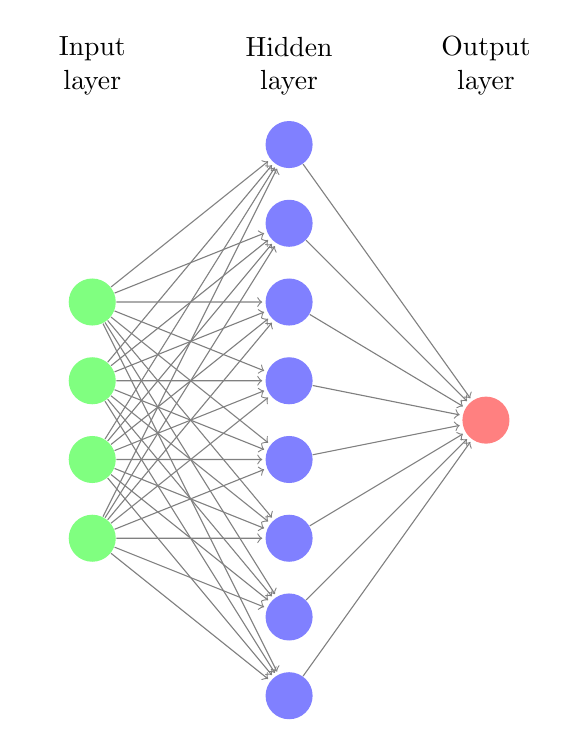
\begin{tikzpicture}[shorten >=1pt,->,draw=black!50, node distance=\layersep]
      \tikzstyle{every pin edge}=[<-,shorten <=1pt]
      \tikzstyle{neuron}=[circle,fill=black!25,minimum size=17pt,inner sep=0pt]
      \tikzstyle{input neuron}=[neuron, fill=green!50];
      \tikzstyle{output neuron}=[neuron, fill=red!50];
      \tikzstyle{hidden neuron}=[neuron, fill=blue!50];
      \tikzstyle{annot} = [text width=4em, text centered]

      % Draw the input layer nodes
      \foreach \name / \y in {1,...,4}
      % This is the same as writing \foreach \name / \y in {1/1,2/2,3/3,4/4}
      \node[input neuron] (I-\name) at (0,-\y) {};

      % Draw the hidden layer nodes
      \foreach \name / \y in {1,...,8}
          \path[yshift=2.0cm]
              node[hidden neuron] (H-\name) at (\layersep,-\y cm) {};

      % Draw the output layer node
      \node[output neuron, right of=H-5,yshift=0.5cm] (O) {};

      % Connect every node in the input layer with every node in the
      % hidden layer.
      \foreach \source in {1,...,4}
          \foreach \dest in {1,...,8}
              \path (I-\source) edge (H-\dest);

      % Connect every node in the hidden layer with the output layer
      \foreach \source in {1,...,8}
          \path (H-\source) edge (O);

      % Annotate the layers
      \node[annot,above of=H-1, node distance=1cm] (hl) {Hidden layer};
      \node[annot,left of=hl] {Input layer};
      \node[annot,right of=hl] {Output layer};
  \end{tikzpicture}\\
\end{center}
\caption{A single-layer feed-forward neural network with $n=4$ and $N=8$}
\label{fig:nn}
\end{figure}

\subsection{Universal Approximator}

In this section we will study the different subsets on which the logistic and ReLU functions act as universal approximators.\\ 

\subsubsection{Sigmoidal functions}

We say that a function $\sigma \in \F(I_n, \R)$ is a sigmoidal function if:

\begin{center}
  $\sigma(x) \to
  \begin{cases}
    0 &\text{as $t \to +\infty$}\\
    1 &\text{as $t \to -\infty$}
  \end{cases}$
\end{center}

The sigmoidal functions include the logistic function defined as:

\begin{center}
  $f(x) = \frac{1}{1+e^{-x}}$
\end{center}

widely used as an activation function for neural networks.\\

The first study of neural network expressiveness with sigmoidal functions dates back to by G.Cybenko in 1989 \cite{cybenko_approximation_1989}. He proved that $S_\sigma$ for $\sigma$ a sigmoidal function is dense in regards of the supremum norm in $C(I_n, \R)$. The demonstration goes as follows.\\

We denote $M(I_n)$ the space of signed regular Borel measures on $I_n$\\

\begin{definition}
  $\sigma$ \text{is discriminatory if} $\mu \in M(I_n)$ \text{and}\\ 
  \begin{center}
  $\forall y \in \R^n,$ $\theta \in \R \int\limits_{I_n} \sigma(y^Tx + \theta) d\mu(x) = 0 \implies \mu = 0$
\end{center}
\end{definition}

\begin{theorem}
  Let $\sigma$ be a contininuous discriminatory function. Then finite sums of the form\\\begin{center}
    $G(x) = \sum\limits_{i=1}^N \alpha_i \sigma(y^Tx + \theta_i)$
  \end{center}
  are dense in $C(I_n, \R)$
\end{theorem}

\begin{proof}
  Let $S \subset C(I_n)$ be the set of the function of the form $G(x)$. S is a linear subset of $C(I_n)$. Let us show that the closure of $S$ is $C(I_n)$.\\

  Assume it is not the case. Then the closure of $S$, denoted $R$, is a proper subspace of $C(I_n)$. Using the Hahn-Banach theorem, there exists $L$ a bounded linear functional on $C(I_n)$ with $L \ne 0$ and  $L(R) = L(S) = 0$\\

  Using the Riesz representation theorem, we obtain:
  \begin{center}
    $L(h) = \int\limits_{I_n} h(x)d\mu(x)$
  \end{center}
  for some $\mu \in M(I_n)$, for all $h\in C(I_n)$. Since $\sigma(y^Tx + \theta_i)  \in R$, we have
  \begin{center}
    $\forall y, \theta \int\limits_{I_n} \sigma(y^Tx + \theta) d\mu(x) = 0$
  \end{center}
  Since $\sigma$ is discriminatory, we have $\mu = 0$ and $L = 0$ follows!\\
  
  Therefore the closure of $S$ is $C(I_n)$ and by definition $S$ is dense in $C(I_n)$
\end{proof}\\
\Sv
  Now let us show that sigmoidal functions are discriminatory.
  \begin{lemma}
    Any bounded, measurable sigmoidal function, a, is discriminatory. In particular, any continuous sigmoidal function is discriminatory.
  \end{lemma}

  \begin{proof}
    First note $\forall x,y,\theta, \phi$ 
\begin{center}
  $\sigma_\lambda(x) = \sigma(\lambda (y^Tx + \theta) + \phi)
  \begin{cases}
    \to 1 &\text{for $y^Tx+\theta > 0$ as $\lambda \to +\infty$}\\
    \to 0 &\text{for $y^Tx+\theta < 0$ as $\lambda \to +\infty$}\\
    =\sigma(\phi) & \text{for $y^Tx+\theta = 0$}
  \end{cases}$
\end{center}
Thus $\sigma_\lambda(x)$ converges pointwise and boundedly to:

\begin{center}
  $\gamma(x)
  \begin{cases}
    =1 &\text{for $y^Tx+\theta > 0$}\\
    =0 &\text{for $y^Tx+\theta < 0$}\\
    =\sigma(\phi) & \text{for $y^Tx+\theta = 0$}
  \end{cases}$
\end{center}
as $\lambda \to +\infty$\\
\sv
Let $\Pi_{y,\theta} = \{x \mid y^Tx+\theta = 0\}$ and let $H_{y,\theta} = \{x \mid y^Tx + \theta > 0\}$. Lesbegue bounded convergence theorem gives us:
\begin{center}
  $0 = \int\limits_{I_n}\sigma_\lambda(x)d\mu(x)$\\
  $ = \int\limits_{I_n} \gamma(x)d\mu(x)$\\
  $\sigma(\phi)\mu(\Pi_{y,\theta}) + \mu(H_{y,\theta})$
\end{center}
for all $\phi, \theta, y$\\
\sv
Fix $y$, we write
\begin{center}
  $F(h) = \int_{I_n}h(y^Tx)d\mu(x)$
\end{center}
Note that $F$ is a bounded function on $L^\infty(\R)$ since $\mu$ is a signed mesure. By chosing  $h$ as the indicator function on $[\theta, \infty[$, we have:
\begin{center}
  $F(h) = \int_{I_n} h(y^Tx) d\mu(x) = \mu(\Pi_{y,-\theta}) + \mu(H_{y,-\theta}) = 0$
\end{center}
By linearity $F(h) = 0$ for indicator functions on any interval and hence for any simple function (sum of indicator functions). Since simple functions are dense in $L^{\infty}(\R), F = 0$.
In particular it is true for the bounded functions $s(u) = sin(m.u)$ and $c(u) = cos(m.u)$. It gives:
\begin{center}
  $F(s+ic) = \int_{I_n} cos(m^Tx) + i sin(m^Tx) d\mu(x) = \int_{I_n} exp(im^Tx)d\mu(x) = 0$
\end{center}
for all $m$. Therefore the fourier transform of $\mu$ is 0 and $\mu$ must be 0. Hence $\sigma$ is discriminatory.
  \end{proof}\\

  This proves that any function of $C(I_n, \R)$ can be approximated by a single-layer network with sigmoidal functions as activation function.\\

  In 1991, Hornik extended in \cite{hornik_approximation_1991} Cybenko's theorem giving the proof for bounded non-constant functions of $F(I_n,\R)$. The proof is very similar to the original one.\\

\subsubsection{ReLU functions}

ReLU functions stands for Rectified Linear Units, there are formed of two pieces of linear functions. They gained interest recently by showing convincing results in a lot of different applications.\\ 

In 2016 Arora et al. \cite{arora_understanding_2018} showed a version of the universal approximation theorem for piecewise linear function that includes ReLU functions.\\

\begin{definition}
  We say a function $f: \R^n \to \R$ is continuous piecewise linear (PWL) if there exists a finite set of polyhedra whose union is $\R^n$, and $f$ is affine linear over each polyhedron (implies continuity because affine regions are closed and cover $\R^n$)
\end{definition}

\begin{proposition}
  Every function in $L^q(\R^n), (1 \le q \le \infty)$ can be arbitrarily approximated in the $L^q$ norm (which for a function $f$ is given by $||f||_q = (\int |f|^q)^{1/q}$) by a ReLU Deep Neural Network.
\end{proposition}

\begin{proof}

  We know that any ReLU DNN represents a PWL function, let's prove the converse.\\
  \sv
  By theorem 1 in \cite{wang_generalization_2005} any piecewise linear function $f: \R^n \to \R$, can be written:
  \begin{center}
    $f = \sum\limits_{j=1}^{p}s_j(\max\limits_{i\in S_j} l_i)$
  \end{center}
  with $l_i$ $(i\le i \le k)$ linear functions, $S_i$ $(1 \le i \le p) \subseteq \{1, ..., k\}$ with $\forall i, |S_i| \le n + 1$ and $\forall j \in \{1,...,p\},  s_j \in \{-1, +1\}$ \\
  \sv
  It means that any PWL convex function can be represented as a linear combination of at most $n+1$ affine pieces, i.e. a ReLU DNN with size $n+1$.\\
  \SV
  Let $p \in \N^*$, let $f \in L^p(\R^n)$, consider the function sequence:
  \begin{center}
    $f_n(x) = (x - \frac{k}{n})f(\frac{k}{n}) + (1 - x + \frac{k}{n})f(\frac{k+1}{n})$ with $\frac{k}{n} \le x < \frac{k+1}{n}, n \ge 1$ 
  \end{center}

  $f_n \xrightarrow[n \to \infty]{} f$, and $\forall n, f_n$ is a PWL continous function. Therefore the continuous PWL functions are dense in $L^p(\R^n)$.
  \SV
  Since any PWL function $\R^n \to \R$ is representable by a ReLU DNN, unniversal approximation theorem follows from the fact that the family of continuous PWL functions is dense in any $L^p(\R^n)$ space for $1 \le p \le \infty$. 
  
\end{proof}\\
\SV
In this article, Arora et al. also gave a higher bound for the depth of the network. They showed that the network required for any function $f \in L^q(\R^n)$ is of at most depth $\lceil log_2(n+1) \rceil$.\\

In 2018, Hannin \& Selke \cite{hanin_approximating_2018} showed that the minimal width a ReLU neural network must have in order to approximate any function $f: \R^n \to \R^m$ a depth $d \ge n + m$ giving a lower bound to the width of the ReLU network.

\newpage
\thispagestyle{empty}
\mbox{}
\newpage

\section{Mathematical preliminaries}

\subsection{Homology}
\label{sec:homology}

The study of homology is part of the field of algebraic topology. We will first introduce the concept of homology, then take a look at the theoretical concept behind it by introducing $\Delta$-complexes: a primitive topological structure that allows the study of homology. Then with the introduction of simplicial homology we will complete the presentation of the fundamental objects used in our research in the study of homology. We will then reconsider these tools in the context of our research. This part heavily relies on the book \textit{Algebraic Topolgy} by A. Hatcher \cite{hatcher_algebraic_2002} and the class given by P. Albin at University of Illinois \cite{albin_1_2018} with the same book as class material. 

\subsubsection{The idea of homology}

In algebraic topology, the most fundamental object to study is the homotopy, that roughly studies "paths". This study leads to the definition of the fundamental group $\pi_1(X)$ that gives information on the topological stucture of a space $X$ for low-dimensional space. However the fundamental group $\pi_1(X)$ can not for instance distinguish the different spheres $\mathcal{S}^n, n\ge 2$. A workaround for that problem is to generalize the notion of homotopy to higher dimensions with different groups $\pi_n(X)$ generalizing the concept of homotopy in higher dimension. \\

However the homotopy groups suffers a serious drawback in their difficult computationality for high dimensions. Even for simple spaces like spheres, the calculation of $\pi_i(\mathcal{S}^n)$ turns out to be very difficult for $i > n$. That is why homology exists as a computable alternative homotopy.\\

\begin{center}
  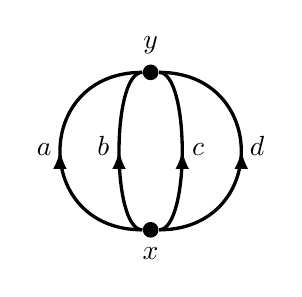
\begin{tikzpicture}[node distance={20mm}] 
    \node[circle,fill,inner sep=2pt, label=below:{$x$}] (1) {}; 
    \node[circle,fill,inner sep=2pt, label=above:{$y$}] (2) [above of=1] {}; 
\begin{scope}[very thick,decoration={
    markings,
    mark=at position 0.5 with {\arrow{latex}}}
    ] 
    \draw[postaction={decorate}] (1) .. controls +(left:1.5cm) and +(left:1.5cm) .. (2)
\foreach \p in {$a$} {node[sloped,above,pos=0.5,rotate=-90, xshift=-0.2cm, yshift=-0.2cm]{\p}};
 \draw[postaction={decorate}, fill=white] (1) .. controls +(left:0.5cm) and +(left:0.5cm) .. (2)
\foreach \p in {$b$} {node[sloped,above,pos=0.5,rotate=-90, xshift=-0.2cm, yshift=-0.2cm]{\p}};
 \draw[postaction={decorate}] (1) .. controls +(right:0.5cm) and +(right:0.5cm) .. (2)
\foreach \p in {$c$} {node[sloped,above,pos=0.5,rotate=-90, xshift=0.2cm, yshift=-0.2cm]{\p}};
 \draw[postaction={decorate}] (1) .. controls +(right:1.5cm) and +(right:1.5cm) .. (2)
\foreach \p in {$d$} {node[sloped,above,pos=0.5,rotate=-90, xshift=0.2cm, yshift=-0.2cm]{\p}};
\end{scope}
\end{tikzpicture} 
\end{center}

Consider the space $X_1$ in the figure drawn above. We can see two points $x$ and $y$ as well as four edges $a$, $b$, $c$ and $d$. Consider the loops formed by travelling along the edges, for instance the path $ab^{-1}$ is a loop with $x$ as the basepoint. Something to consider is that the loop $b^{-1}a$ is basically the same loop but starting from a different basepoint, $y$ in that case. By abelianizing, we can consider cycles instead of loops without any basepoint.\\

The abelian groups having only one operation, we will then switch to additive notations to remain in accordance with Hatcher's notations. With that new notation we can write equalities such as $(a-c) + (b-d) = (a-d) + (b-c)$. This is justified by the fact that from an algebraic point of view, there is no difference between these two cycles.\\

Let us call any linear combination of edges, \textit{chains}. Then the condition for a chain $ka + lb + mc + nd$ with $k,l,m,n \in \N$ to be a cycle is $k + l + m + n = 0$.\\

Now let us start to formalize these concepts. Consider $C_0$ the free abelian group spanned by the vertices $x,y$ and let $C_1$ be the free abelian group spanned by the edges $a,b,c,d$. One can define an homomorphism $\delta: C_1 \to C_0$ that sends any basis element of $C_1$ to $x-y$. Thus we have $\delta(ka+lb+mc+nd) = (k+l+m+n)a - (k+l+m+n)y$ and $ker(\delta) = \{$ cycles of $X_1$ $\}$. $\{ a-b, b-c, c-d \}$ forms a basis for this kernel, i.e. any cycle is a linear combination of the most obvious cycles of $X_1$, that conveys the information that $X_1$ has three visibles "holes" formed by the space between its four edges.\\

\begin{center}
  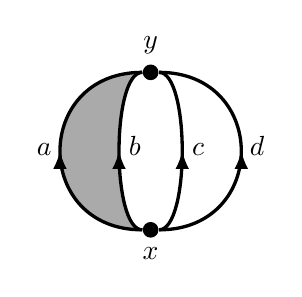
\begin{tikzpicture}[node distance={20mm}] 
    \node[circle,fill,inner sep=2pt, label=below:{$x$}] (1) {}; 
    \node[circle,fill,inner sep=2pt, label=above:{$y$}] (2) [above of=1] {}; 
\begin{scope}[very thick,decoration={
    markings,
    mark=at position 0.5 with {\arrow{latex}}}
    ] 
    \draw[postaction={decorate}, fill={rgb:black,1;white,2}] (1) .. controls +(left:1.5cm) and +(left:1.5cm) .. (2)
      \foreach \p in {$a$} {node[sloped,above,pos=0.5,rotate=-90, xshift=-0.2cm, yshift=-0.2cm] (3) {\p}};
 \draw[postaction={decorate}, fill=white] (1) .. controls +(left:0.5cm) and +(left:0.5cm) .. (2)
   \foreach \p in {$b$} {node[sloped,above,pos=0.5,rotate=-90, xshift=0.2cm, yshift=-0.2cm] (4) {\p}};
 \draw[postaction={decorate}] (1) .. controls +(right:0.5cm) and +(right:0.5cm) .. (2)
\foreach \p in {$c$} {node[sloped,above,pos=0.5,rotate=-90, xshift=0.2cm, yshift=-0.2cm]{\p}};
 \draw[postaction={decorate}] (1) .. controls +(right:1.5cm) and +(right:1.5cm) .. (2)
\foreach \p in {$d$} {node[sloped,above,pos=0.5,rotate=-90, xshift=0.2cm, yshift=-0.2cm]{\p}};
\end{scope}
\end{tikzpicture} 
\end{center}

Now fill the hole between edges $a$ and $b$ with a 2-cell, namely $A$ to create a new space $X_2$. Considering it as being oriented clockwise, its boundary is $a-b$. The cycle $a-b$ is homotopic to a point since it can now be contracted by sliding over $A$, it no longer encloses a hole in G. That suggests that homology should consider only the quotient group of what we found previously by $a-b$. In this quotient group the cycles $a-c$ and $b-c$ are equivalent. Which is consistent with the fact that they are homotopic in $X_2$.\\

Algebraically we can now consider a pair of homomorphism $\delta_1, \delta_2$ such that $C_2 \xrightarrow{\delta_2} C_1 \xrightarrow{\delta_1} C_0$ where $C_2$ is the cyclic group spanned by $A$ and $\delta_2(A) = a-b$. The quotient group we are interested in is $ker(\delta_1)/Im(\delta_2)$, i.e. the 1-dimensional cycles modulo those that are boundaries. We will call it the homology group $H_1(X_2)$. It can also be computed in $X_1$ by considering $C_2$ to be zero since there are no 2-cells in $X_1$. $H_1(X_2)$ now only admits two generators $b-c$ and $c - d$ expressing the geometric fact that the number of holes reduced from 3 to 2.\\


\begin{center}
  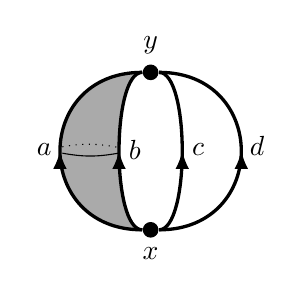
\begin{tikzpicture}[node distance={20mm}] 
    \node[circle,fill,inner sep=2pt, label=below:{$x$}] (1) {}; 
    \node[circle,fill,inner sep=2pt, label=above:{$y$}] (2) [above of=1] {}; 
\begin{scope}[very thick,decoration={
    markings,
    mark=at position 0.5 with {\arrow{latex}}}
    ] 
    \draw[postaction={decorate}, fill={rgb:black,1;white,2}] (1) .. controls +(left:1.5cm) and +(left:1.5cm) .. (2)
      \foreach \p in {$a$} {node[sloped,above,pos=0.5,rotate=-90, xshift=-0.2cm, yshift=-0.2cm] (3) {\p}};
 \draw[postaction={decorate}, fill=white] (1) .. controls +(left:0.5cm) and +(left:0.5cm) .. (2)
   \foreach \p in {$b$} {node[sloped,above,pos=0.5,rotate=-90, xshift=0.2cm, yshift=-0.25cm] (4) {\p}};
 \draw[postaction={decorate}] (1) .. controls +(right:0.5cm) and +(right:0.5cm) .. (2)
\foreach \p in {$c$} {node[sloped,above,pos=0.5,rotate=-90, xshift=0.2cm, yshift=-0.2cm]{\p}};
 \draw[postaction={decorate}] (1) .. controls +(right:1.5cm) and +(right:1.5cm) .. (2)
\foreach \p in {$d$} {node[sloped,above,pos=0.5,rotate=-90, xshift=0.2cm, yshift=-0.2cm]{\p}};
\end{scope}
\draw[dotted] (3) to [out=10, in=170] (4);
\draw (3) to [out=350, in=190] (4);
\end{tikzpicture} 
\end{center}

Suppose we attach another 2-cell between $a$ and $b$ to create $X_3$, namely $B$. $C_2$ now consists of linear combinations of $A$ and $B$ and $\delta_2(A) = \delta_2(B) = a-b$. On the one hand, $H_1(X_3) = H_1(X_2) \approx \Z \times \Z$, but on the other hand $ker(\delta_2) \neq 0$ and $A-B$ is its generator, hence we have $H_2(X_3) = ker(\delta_2) \approx \Z$. Topologically the cycle $A-B$ is equivalent to a sphere and it detects the presence of a "hole" enclosed by this sphere rather than a circle.\\

The pattern we can see appear with these examples is rather clear. The n-cell complexes of $X$ forms free abelian groups $C_n(X)$ and one can define homomorphisms $\delta_n: C_n \to C_{n-1}$ to define homology groups $H_n(X) = ker(\delta_n)/Im(\delta_{n+1})$. The only problem now is to define $\delta_n$ for any $n$. If it is simple for small $n$ (head minus tail for a vertex), it becomes rather complicated when $n$ grows and more complex polyhedral cells appear in $X$. The most efficient approach is to decompose polyhedra into simplices which allows simple orientation and boundary computation. For that purpose we will define nice cellular complexes that will be the fundamental element for homology computation in the homology theories presented after. 

\subsubsection{$\Delta$-complexes}
\label{sec:delta_complexes}

The most important theory of algebraic topology is called singular homology, since it is technically complicated we will use a simpler version of it called simplicial homology. The natural definition spaces of simplicial homology is called $\Delta$-complexes that we will introduce in this part.\\

The projective plane, the klein bottle and the torus can be obtained from squares by identifying edges and giving them orientation as draw below.

\tcbset{top=0pt,right=10pt,left=10pt,bottom=0pt,nobeforeafter, colframe=blue!75!black,colback=white,fonttitle=\bfseries,center title}
\begin{center}
  \tcbox[title=$T$]{
  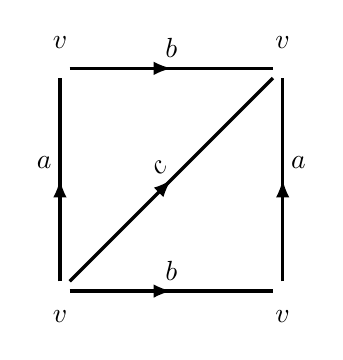
\begin{tikzpicture}[node distance={20mm}] 
    \node[draw=none, label={}] (1) {}; 
    \node[draw=none, label={$v$}] (2) [above right of=1] {}; 
    \node[draw=none, label={$v$}] (3) [above left of=1] {}; 
    \node[draw=none, label=below:{$v$}] (4) [below right of=1] {}; 
    \node[draw=none, label=below:{$v$}] (5) [below left of=1] {}; 
\begin{scope}[very thick,decoration={
    markings,
    mark=at position 0.5 with {\arrow{latex}}}
    ] 
    \draw[postaction={decorate}] (3) -- (2)
      \foreach \p in {$b$} {node[sloped,above,pos=0.5,rotate=0] (6) {\p}};
    \draw[postaction={decorate}] (4) -- (2)
      \foreach \p in {$a$} {node[sloped,above,pos=0.5,rotate=-90, xshift=0.2cm] (7) {\p}};
    \draw[postaction={decorate}] (5) -- (4)
      \foreach \p in {$b$} {node[sloped,above,pos=0.5,rotate=0] (8) {\p}};
    \draw[postaction={decorate}] (5) -- (3)
      \foreach \p in {$a$} {node[sloped,above,pos=0.5,rotate=-90, xshift=-0.2cm] (9) {\p}};
    \draw[postaction={decorate}] (5) -- (2)
      \foreach \p in {$c$} {node[sloped,above,pos=0.5,rotate=0] (10) {\p}};
\end{scope}
      
\end{tikzpicture} 
}
\hspace{0.0cm}
\tcbox[title=$\R P^2$]{
  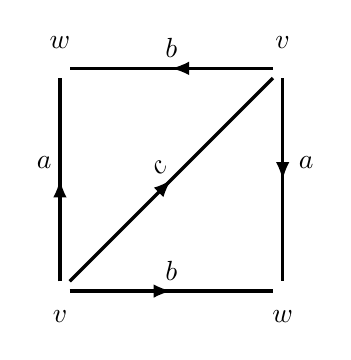
\begin{tikzpicture}[node distance={20mm}] 
    \node[draw=none, label={}] (1) {}; 
    \node[draw=none, label={$v$}] (2) [above right of=1] {}; 
    \node[draw=none, label={$w$}] (3) [above left of=1] {}; 
    \node[draw=none, label=below:{$w$}] (4) [below right of=1] {}; 
    \node[draw=none, label=below:{$v$}] (5) [below left of=1] {}; 
\begin{scope}[very thick,decoration={
    markings,
    mark=at position 0.5 with {\arrow{latex}}}
    ] 
    \draw[postaction={decorate}] (2) -- (3)
      \foreach \p in {$b$} {node[sloped,above,pos=0.5,rotate=0] (6) {\p}};
    \draw[postaction={decorate}] (2) -- (4)
      \foreach \p in {$a$} {node[sloped,above,pos=0.5,rotate=90, xshift=0.3cm] (7) {\p}};
    \draw[postaction={decorate}] (5) -- (4)
      \foreach \p in {$b$} {node[sloped,above,pos=0.5,rotate=0] (8) {\p}};
    \draw[postaction={decorate}] (5) -- (3)
      \foreach \p in {$a$} {node[sloped,above,pos=0.5,rotate=-90, xshift=-0.2cm] (9) {\p}};
    \draw[postaction={decorate}] (5) -- (2)
      \foreach \p in {$c$} {node[sloped,above,pos=0.5,rotate=0] (10) {\p}};
\end{scope}
\end{tikzpicture}
}
\hspace{0.0cm}
\tcbox[title=$K$]{
  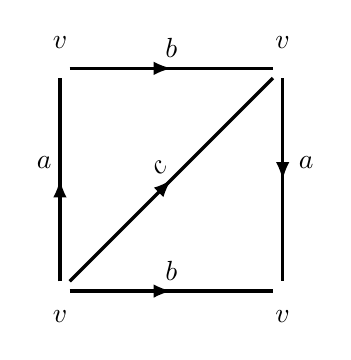
\begin{tikzpicture}[node distance={20mm}] 
    \node[draw=none, label={}] (1) {}; 
    \node[draw=none, label={$v$}] (2) [above right of=1] {}; 
    \node[draw=none, label={$v$}] (3) [above left of=1] {}; 
    \node[draw=none, label=below:{$v$}] (4) [below right of=1] {}; 
    \node[draw=none, label=below:{$v$}] (5) [below left of=1] {}; 
\begin{scope}[very thick,decoration={
    markings,
    mark=at position 0.5 with {\arrow{latex}}}
    ] 
    \draw[postaction={decorate}] (3) -- (2)
      \foreach \p in {$b$} {node[sloped,above,pos=0.5,rotate=0] (6) {\p}};
    \draw[postaction={decorate}] (2) -- (4)
      \foreach \p in {$a$} {node[sloped,above,pos=0.5,rotate=90, xshift=0.3cm] (7) {\p}};
    \draw[postaction={decorate}] (5) -- (4)
      \foreach \p in {$b$} {node[sloped,above,pos=0.5,rotate=0] (8) {\p}};
    \draw[postaction={decorate}] (5) -- (3)
      \foreach \p in {$a$} {node[sloped,above,pos=0.5,rotate=-90, xshift=-0.2cm] (9) {\p}};
    \draw[postaction={decorate}] (5) -- (2)
      \foreach \p in {$c$} {node[sloped,above,pos=0.5,rotate=0] (10) {\p}};
\end{scope}
\end{tikzpicture}
}
\end{center}

In fact any closed surface can be constructed this way, i.e. by cutting a polygon along its diagonals and identifying pairs of edges. The idea between $\Delta$-complexes is to generalize this idea to any dimension. The n-dimensional analog of the triangle is called the n-simplex.This is the smallest convex set in a Euclidean space $\R^m$ containing $n + 1$ points $v_0 , ... , v_n$ that do not lie in a hyperplane of dimension less than $n$. The points $v_i$ are the vertices of the simplex and the simplex is denoted $[v_0, ..., v_n]$. The standard n-simplex is:\\

\begin{center}
  $\Delta^n = \{ (t_0,...t_n) \in \R^{n+1} \mid \sum_i t_i  = 1$ and $t_i \ge 0$ for all $i \}$
\end{center}

Its vertices are the unit vectors along the coordinate axes.\\

It is important to keep track of an ordering for the vertices and an n-simplex will always be considered with an ordering for its vertices. That will allow us to give an orientation for its edges $[v_iv_j]$ with respect to the ordering of the indices. It also determines a canonical linear homeomorphism from the standard n-simplex $\Delta^n$ into any other n-simplex preserving the order of the vertices: $(t_0, ..., t_n) \mapsto \sum_i t_i v_i$. The coefficients are the barycentric coordinates of the points $\sum_i t_i v_i$ in $[v_0, ..., v_n]$.\\

If we delete one of the vertices of an n-simplex $[v_0, ..., v_n]$, the remaining n vertices span an (n-1)-simplex, called face of $[v_0, ..., v_n]$ that will conventionnaly keep the same orientation as in $[v_0, ..., v_n]$. The union of all the face of $\Delta^n$ is the boundary of $\Delta^n$, noted $\delta \Delta^n$. The open simplex $\mathring{\Delta}^n$ is $\Delta^n - \delta \Delta^n$, is the interior of $\Delta^n$.\\

A $\Delta$-complex on a topological space $X$ is a collection of maps $\sigma_\alpha : \Delta^n \to X$  with the following properties:\\

\begin{enumerate}[label=(\roman*)]
  \item The restriction $\sigma_\alpha \mid \mathring{\Delta}^n$ is injective, and each point of $X$ is in the image of exactly one such restriction $\sigma_\alpha \mid \mathring{\Delta}^n$.
  \item Each restriction if $\sigma_\alpha$ to a face of $\Delta^n$ is one if the maps $\sigma_\beta : \Delta^{n-1} \to X$ (identifying the face of $\Delta^n$ with the face of $\Delta^{n-1}$ using the canonical linear homeomorphism between them and preserving the vertices ordering).
  \item A set $A \subset X$ is open if and only if $\sigma_\alpha^{-1}(A)$ is open in $\Delta^n$ for each $\sigma_\alpha$.
\end{enumerate}

The earlier decompositions of the torus, projective plane, and Klein bottle into two triangles, three edges, and one or two vertices allow well-definess of associated $\Delta$-complex structures with a total of six $\sigma_\alpha$'s for the torus and Klein bottle and seven for the projective plane. The orientation of edges are compatible with an ordering of the vertices (example below). This ordering determines the maps $\sigma_\alpha$.

\begin{figure}[H]
\begin{center}
\tcbox[title=$T$]{
  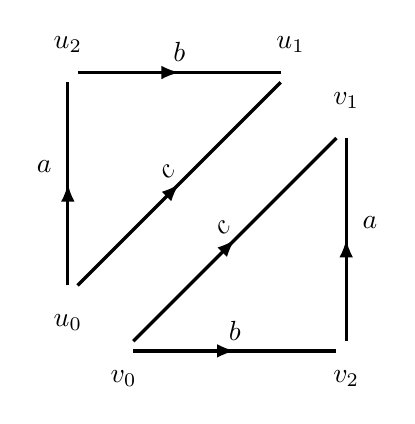
\begin{tikzpicture}[node distance={10mm}] 
    \node[draw=none, label={}] (1) {}; 
    \node[draw=none, label={}] (2) [below left of=1] {}; 
    \node[draw=none, label={}] (3) [below right of=1] {}; 
    \node[draw=none, label={}] (4) [above right of=1] {}; 
    \node[draw=none, label=below:{$v_0$}] (5) [below left of=2] {}; 
    \node[draw=none, label=below:{$v_2$}] (6) [below right of=3] {}; 
    \node[draw=none, label={$v_1$}] (7) [above right of=4] {}; 
    \node[draw=none, label={}] (8) [above left of=1] {}; 
    \node[draw=none, label={}] (9) [below left of=8] {}; 
    \node[draw=none, label={}] (10) [above left of=8] {}; 
    \node[draw=none, label={}] (11) [above right of=8] {}; 
    \node[draw=none, label={$u_1$}] (12) [above right of=11] {}; 
    \node[draw=none, label={$u_2$}] (13) [above left of=10] {}; 
    \node[draw=none, label=below:{$u_0$}] (14) [below left of=9] {}; 
\begin{scope}[very thick,decoration={
    markings,
    mark=at position 0.5 with {\arrow{latex}}}
    ] 
    \draw[postaction={decorate}] (5) -- (6)
      \foreach \p in {$b$} {node[sloped,above,pos=0.5,rotate=0] (17) {\p}};
    \draw[postaction={decorate}] (6) -- (7)
      \foreach \p in {$a$} {node[sloped,above,pos=0.5,rotate=-90, xshift=0.3cm] (15) {\p}};
    \draw[postaction={decorate}] (5) -- (7)
      \foreach \p in {$c$} {node[sloped,above,pos=0.5,rotate=0] (16) {\p}};
    \draw[postaction={decorate}] (14) -- (13)
      \foreach \p in {$a$} {node[sloped,above,pos=0.5,rotate=-90, xshift=-0.3cm] (18) {\p}};
    \draw[postaction={decorate}] (13) -- (12)
      \foreach \p in {$b$} {node[sloped,above,pos=0.5,rotate=0] (19) {\p}};
    \draw[postaction={decorate}] (14) -- (12)
      \foreach \p in {$c$} {node[sloped,above,pos=0.5,rotate=0] (20) {\p}};
\end{scope}
\end{tikzpicture}
}
\end{center}
\caption{The $\delta$-complex structure of the torus $T$}
\label{fig:delta_torus}
\end{figure}

\subsubsection{Simplicial homology}

Let us now define the simplicial homology groups of a $\Delta$-complex $X$. Let $\Delta_n(X)$ be the free abelian group with basis the open $n$-simplices $e^n_\alpha$ of $X$. The elements of $\Delta_n(X)$ are called n-chains and are of the form $\sum_\alpha n_\alpha e^n_\alpha$ with $n_\alpha \in \Z$. Equivalently, this could be written as $\sum_\alpha n_\alpha \sigma_\alpha$ where $\sigma_\alpha : \Delta^n \to X$ is the characteristic map of $e^n_\alpha$ with image the closure of $e^n_\alpha$. Such a sum can be considered as a finite collection, or "chain", of $n$-simplices in $X$.\\

The boundary of the $n$-simplex $[v_0, ..., v_n]$ consists of the various $(n-1)$-dimensional simplices $[v_0, ... , \hat{v_i} , ... , v_n]$ (indicates all $v_{k}, 1 \le k \le n$ but $i$). We might wish that the boundary of  $[v_0, ..., v_n]$ be the $(n-1)$-chain formed by the sum of the faces $[v_0, ... ,\hat{v_i} , ... , v_n]$. It turns out to be betters to insert sign to take into account orientations. It allow to coherently orient all the faces of the simplex. That is why we let the boundary be $\sum_i (-1)^i [v_0, ... , \hat{v_i} , ... , v_n]$.\\


\tcbset{colback=white,colframe=black,top=10mm,bottom=10mm}
\begin{tcolorbox}
\begin{multicols}{2}
  \begin{center}
  \begin{tikzpicture}[node distance={20mm}] 
    \node[draw=none, label={}] (1) {}; 
    \node[draw=none, label=right:{$v_1$}] (2) [above right of=1] {}; 
    \node[draw=none, label=left:{$v_0$}] (3) [above left of=1] {}; 
\begin{scope}[very thick,decoration={
    markings,
    mark=at position 0.5 with {\arrow{latex}}}
    ] 
    \draw[postaction={decorate}] (3) -- (2)
      \foreach \p in {} {node[sloped,above,pos=0.5,rotate=90, xshift=0.3cm] (5) {\p}};
\end{scope}
\end{tikzpicture}
\\
  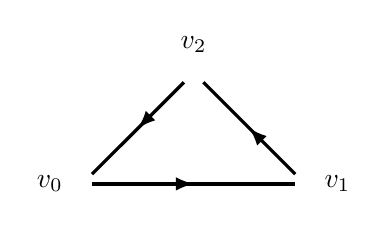
\begin{tikzpicture}[node distance={20mm}] 
    \node[draw=none, label={$v_2$}] (1) {}; 
    \node[draw=none, label=right:{$v_1$}] (2) [below right of=1] {}; 
    \node[draw=none, label=left:{$v_0$}] (3) [below left of=1] {}; 
\begin{scope}[very thick,decoration={
    markings,
    mark=at position 0.5 with {\arrow{latex}}}
    ] 
    \draw[postaction={decorate}] (1) -- (3)
      \foreach \p in {} {node[sloped,above,pos=0.5,rotate=0] (4) {\p}};
    \draw[postaction={decorate}] (3) -- (2)
      \foreach \p in {} {node[sloped,above,pos=0.5,rotate=90, xshift=0.3cm] (5) {\p}};
    \draw[postaction={decorate}] (2) -- (1)
      \foreach \p in {} {node[sloped,above,pos=0.5,rotate=0] (5) {\p}};
\end{scope}
\end{tikzpicture}
\end{center}
\begin{center}


\columnbreak

$\delta [v_0,v_1] = [v_1] - [v_0]$\\
\vspace{2.3cm}

$\delta [v_0, v_1, v_2] = [v_1, v_2] - [v_0, v_2] + [v_0, v_1]$

\end{center}
\end{multicols}
\end{tcolorbox}
\\

We define a boundary homomorphism for a general $\Delta$-complex $X$, $\delta_n : \Delta_n (X) \to \Delta_{n-1} (X)$ by specifying its values on the basis elements:

\begin{center}

  $\delta_n(\sigma_\alpha) = \sum_i (-1)^i \sigma_\alpha \mid [v_0 , ... , \hat{v_i} , ... , v_n]$

\end{center}

The image set of $\delta_n$ is $\Delta_{n-1} (X)$ since each restriction $\sigma_\alpha \mid [v_0 , ... , \hat{v_i} , ... , v_n]$ is the caracteristic map of an $(n-1)$-simplex of $X$.\\

\begin{lemma}

  The composition $\Delta_n (X) \xrightarrow{\delta_n} \Delta_{n-1} (X) \xrightarrow{\delta_{n-1}} \Delta_{n-2} (X)$ is zero.

  \label{lemma:delta_comp}
\end{lemma}

\begin{proof}

  We have $\delta_n(\sigma) = \sum_i (-1)^i \sigma \mid [v_0, ... , \hat{v_i} , ... , v_n] $, hence \\
  \vspace{-10pt}
  \begin{center}
  $\delta_{n-1}\delta_n (\sigma) = \sum\limits_{j < i} (-1)^i (-1)^j \sigma \mid [v_0, ... , \hat{v_j} , ... , \hat{v_j} , ... , v_n]$
  \sv
$+ \sum\limits_{j > i} (-1)^i (-1)^{j-1} \sigma \mid [v_0, ... , \hat{v_i}, ... , \hat{v_j} , ... , v_n] = 0$.
\end{center}

  The last equality comes from the switch of $i$ and $j$ in the second sum.

\end{proof}
\\

We end up with a sequence of homomorphisms of abelian groups:

\begin{center}
  $... \to C_{n+1} \xrightarrow{\delta_{n+1}} C_n \xrightarrow{\delta_n} C_{n-1} \to ... \to C_1 \xrightarrow{\delta_1} C_0 \xrightarrow{\delta_0} 0$
\end{center}

with $\delta_n\delta_{n+1} = 0$ for each $n$ (cf Lemma \ref{lemma:delta_comp}).We call such a sequence a chain complex. The equation $\delta_n \delta_{n+1} = 0$ is equivalent to the inclusion Im $\delta_{n+1} \subset$ Ker $\delta_n$. We can define the $n^{th}$ homology group of the chain complex to be the quotient group $H_n =$ Ker $\delta_n$/Im $\delta_{n+1}$. The elements of Ker $\delta_n$ are called cycles and elements of Im $\delta_{n+1}$ are called boundaries. Elements of $H_n$ are cosets of Im $\delta_{n+1}$ called homology classes. Two cycles representing the same homology class are said to be homologous, it means their difference is a boundary.\\

In the case of $C_n = \Delta_n(X)$, the homology group Ker $\delta_n$/Im $\delta_{n+1}$ will be denoted $H^\Delta_n(X)$ and called the $n^{th}$ simplicial homology group of $X$. \\

Example: Let us take $X = T$, the torus with the $\Delta$-complex structure pictured in Figure \ref{fig:delta_torus}. For recall, the structure has one vertex $v$, three edges $a, b, c$ and two 2-simplices $U$ and $V$. $\delta_1 = v - v = 0$ so $H_0^\Delta(X) \approx \Z$. Since $\delta_2 U = a + b - c = \delta_2 L$ and $\{a, b, a+ b - c\}$ is a basis for $\Delta_1(T)$, $H_1^\Delta(X) = \frac{\delta_1(X)}{\delta_2(U)}$, it follows that $H_1^\Delta(X) \approx \Z \oplus \Z$ with basis the homology classes $[a]$ and $[b]$. Since there are no 3-simplices, $H_2^\Delta(T)$ is equal to Ker$\delta_2$, which is infinite cyclic generated by $U-L$ since $\delta(pU+qL) = (p+q)(a+b-c) = 0$ iff $p = -q$.\\

Therefore:
\begin{center}
  $H_n^\Delta(X) \approx
  \begin{cases}
    \Z \oplus \Z &\text{for $n=1$}\\
    \Z &\text{for $n=0,2$}\\
    0 &\text{for $n\ge3$}
  \end{cases}$
\end{center}

\begin{proposition}
  For $n \in \N^*, H_n^\Delta(\S^n) \approx \Z$ with $\S^n$ the $n$-dimension sphere.
\end{proposition}
\begin{proof}
A $\Delta$-complex structure can be otained on $\S^n$ by taking two copies of $\Delta^n$ and identifying boundaries using the identity map. Using previous notations, we have Ker$\delta_n$ an infinite cycle generated by $U-L$. Therefore $H_n^\Delta(\S^n) \approx \Z$.
\end{proof}\\

The simplicial homology is defined for simplical complexes. These are the $\Delta$-complexed whose simplices are uniquely determined by their vertices. Each $n$-simplex has $n+1$ distinct vertices and no other $n$-simplex has the same set of vertices. A simplicial complex can be described as a set $X_0$ of vertices and sets $X_n$ of $n$-simplices which are $(n+1)$-elements subsets of $X_0$. It is required that each $(k+1)$-element subset of the vertices of an $n$-simplex in $X_n$ is a $k$-simplex in $X_k$.\\

Compared with $\Delta$-complexes, simplicial complexes require more computation. For example a simplicial complex structure for the torus would require 14 triangles, 21 edges and 7 vertices. It can be shown that any $\Delta$-complex can be subdivided in a simplical complex.\\


It is worth mentionning that simplicial homology has flaws such as the one mentionend before. That is why in the current theory of homology, simplicial homology has been replaced with a more complete theory of homologies named singular homology. The improvements of simplicial homology brought by singular are not useful for our research, that is why we will not be discussing this theory in this paper. The theory is however thoroughly explained in \cite{hatcher_algebraic_2002}.

\subsubsection{Homology in our research}
\label{sec:homology_research}

Our research is concerned with the capacity of neural networks to properly express after training different difficulty of problems depending on their width. There would be different approach to chosing a way to measure this difficulty that would relate to different applied problems. The first approach would be to look at the dimension of the problem.\\

\begin{figure}[h]
  \centering
  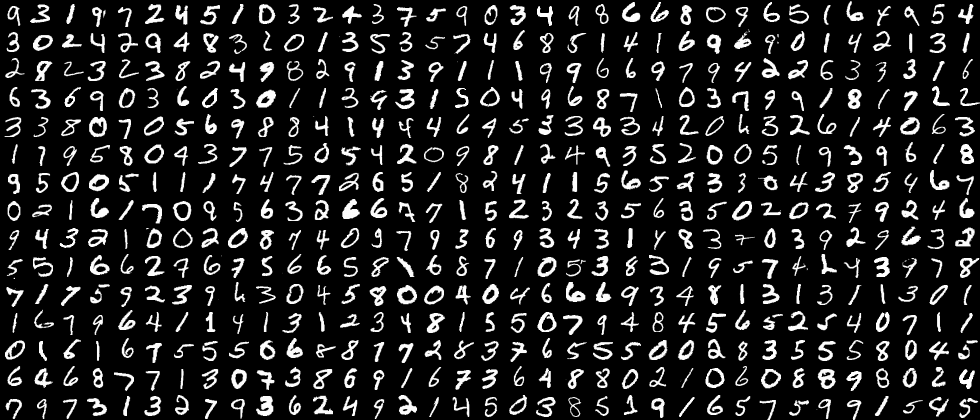
\includegraphics[scale=0.4]{mnist.png}
  \caption{Some images of the MNIST dataset}
  \label{fig:mnist}
\end{figure}

For instance the MNIST problem, aims to classify 28x28 pixels images of handwritten digits in 10 classes representing the 10 digits (see Figure \ref{fig:mnist}). For instance in 2003 in \cite{simard_best_2003}, a team of researcher used a simple neural network of 2 layers with respectively 100 and 10 hidden units to classify the MNIST dataset (they used convolutional layers before inputing data in their network making the input dimension even greater) to obtain an accuracy of 98.81\%. One could expect that solving the same problem of image classification for instance and using different image size and depth of networks would be an interesting way to study the problem of expressiveness.\\

However two major problems occur in that case. First how to choose the classification problem with the certainty that the problem itself is not going to be a problem simpler than it looks? This relates to an hypothesis called the manifold hypothesis. The manifold hypothesis holds roughly as follows: "real-world high-dimensional data lie on low-dimensional manifolds embedded within the high-dimensional space". Meaning that complex data that needs a lot of parameters to be perfectly described are caracterized by few simple parameters up to continuous deformations as defined by topology. Considering this hypothesis that has not been disproved, a certain image recognition problem such as MNIST could be relying on the separation of a space of smaller dimension that the 784 dimensions space that you would expect from 28x28 pixels images.\\

The second problem is the problem of thresholding for accuracy since it is almost impossible to reach 100\%. One would have to chose a value over which one considers the problem as correctly classified and below which it is considered not classified. That choice would be rather arbitrary and it would be hard to evaluate the value of the results as far as they might change radically with a slight change in the choice of the threshold.\\

This point is non-specific to the choice of accuracy as a measure since in any case the training of a neural network is a process with a random component involved and independently of the measure choice, the problem of training artifacts and imprecions might arise. Therefore one should try to chose a measure that will reduce as much as possible this incontrollable component in the research.\\

For that purpose, we have chosen to use homology of the data as our measure. Using homology garantees an independence from the problem chosen since homologies can take different forms due to its topological nature. Moreover if the manifold hypothesis happends to be true, the study of homology in rather small dimension and how neural networks of different depth perform on it might have applications even in high dimension problems. Unlike accuracy the perfect classification in terms of homology is something reachable since homology is studied without regard to continuous deformations ($\approx$ topologically), errors and imprecision will mostly be ignored.\\

\subsection{Topological Data Analysis}

Topological Data Analysis, also called TDA, is an approach to the analysis of datasets using techniques from topology. The idea behind it is to provide with a framework to rigorously study the "shape" of a dataset. The main tool is persistent homology, that allows the computation of homology of a point cloud dataset. This tool will be presented in detail after a general presentation of the field of TDA. This chapter is based on the paper of L. Wasserman \cite{wasserman_topological_2016}. 

\subsubsection{Introduction to TDA method's}

Topological Data Analysis definition is somewhat vague and if it is very clear that persistent homology belong to this field, the exact set of methods, theories and results that belongs to this field is quite imprecise. According to this imprecision we chose to give the following definition to TDA: It's a "large class of data analysis method that uses the notion of shape and connectivity" \cite{wasserman_topological_2016}. In his paper Wasserman details different approaches to this question of shape and conenctivity study starting with density clusters that we will only briefly cover since these methods are of no use for the purpose of our research. We will then in this section present the ideas and tools behind the study of low-dimension support for high dimension sets and their study with TDA's tools. That second part is here in support of the manifold hypothesis discussed briefly in \textbf{Section \ref{sec:homology_research}}.

\paragraph{Density Clustering}

In his paper, Wasserman covers three types of clustering. More clustering methods could be considered as part of TDA but for explanation purposes of what TDA is, the first two methods will be sufficient as they will introduce paradigms we will find in persistent homology.\\

The first method introduced is level set clustering. The idea behind this name is the study of the density of random samples regarding a threshold. Formally consider $X_1, ..., X_n$ a random sample of a distribution $P$ with density $p$ where $X_i \in \mathcal{X} \subset \R^d$.\\

For $t \ge 0$ we define:

  \begin{center}
    $L_t = \lbrace x : p(x) > t \rbrace$
  \end{center}

  The density clusters at level $t$, denoted $C_t$, are the connected components of $L_t$. One can define an estimation of $L_t$, denoted $\hat{L_t}$ as follows:\\
  \begin{center}
    $\widehat{L_t} = \lbrace x : \widehat{p}(x) > t \rbrace $
  \end{center}

  where $\widehat{p}(x)$ is an estimator for the density $p$, such as the kernel density:

  \begin{center}
    $\widehat{p}_h(x) = \frac{1}{n} \sum\limits_{i=1}^n \frac{1}{h^d} K (\frac{||x-X_i||}{h})$
  \end{center}

  where $h > 0$ is the bandwidth and $K$ the kernel.\\

  To find the clusters, one need to find the connected components  of $\widehat{L_t}$. Let $I_t = \lbrace i : \widehat{p_h}(X_i) > t \rbrace$. Create a graph with vertices $(X_i : i \in I_t)$. Now put an edge between two vertices $X_i$ and $X_j$ if $||X_i - X_j|| \le \varepsilon$ where $\varepsilon > 0$ is a parameter ($\varepsilon = 2h$ works well in practice).\\

  It appears the choice of $t$ is crucial in the level set clustering method and there are different possibilities to chose it. First one can chose some prescribed fraction $1-\beta$ of the total mass. Another idea is to look at clusters at all levels $t$. This will lead us to the idea of density trees.\\

  The idea of density trees is to create a concept to study level set clustering for all $t$. That concept will give us both a representation of the structure of the data as well as a way to compare its topological similarity with another set.\\

  The set of all density clusters $\mathcal{C}$ has a tree structure, indeed if $A,B \in \mathcal{C}$ then either $A \subset B$ or $B \subset A$ or $A \cap B = \emptyset$. The tree shows the number of level sets at some level $t$. The number of branches of the tree correponds to the number of connected components. Two density trees have the same "shape" if their tree structure is the same. Given a tree $T_p$ the distance on the tree is defined as: 

  \begin{center}
    $d_{T_p}(x,y) = |p(x) + p(y) - 2m_p(x,y)|$
  \end{center}

  where

  \begin{center}
    $m_p(x,y) = sup \lbrace t : \exists C\in C_i \mid x,y \in C \rbrace$    
  \end{center}
  
  is called the merge height. For any two clusters $C_1, C_2 \in T_p$, we define $\lambda_1 = \lbrace t: C_1 \in C_t \rbrace$ and $\lambda_2$ analogously. We then define the tree distance function on $T_p$ as:

  \begin{center}
    $d_{T_p}(C_1,C_2) = \lambda_1 + \lambda_2 - 2m_p(C_1,C_2)$
  \end{center}

  where

  \begin{center}
    $m_p(C_1,C_2) = sup \lbrace \lambda \in \R : \exists C \in T_p \mid C_1, C_2 \subset C \rbrace$
  \end{center}

  Since $d_{T_p}$ defines a distance on the tree, it induces a topology on $T_p$. Given two densities $p$ and $q$ we can say that $T_p$ is equivalent to $T_q$, denoted $T_p \approx T_q$ if there exists an homeomorphism between the two trees.

\paragraph{Low dimensional subsets}

The point of study of low dimensional subset relates to the manifold hypothesis and more generally the study of the support of the distribution $P$ when it is only a set $S$ of dimension $r$ with $r < d$ (see Figure \ref{fig:swiss_roll}). Sometimes the support of $P$ is of dimension exactly $d$ but there exists a set $S$ of dimension $r < d$ which has a high concentration of mass (see Figure \ref{fig:high_concentration}).\\  

  \begin{figure}[p]
    \centering
  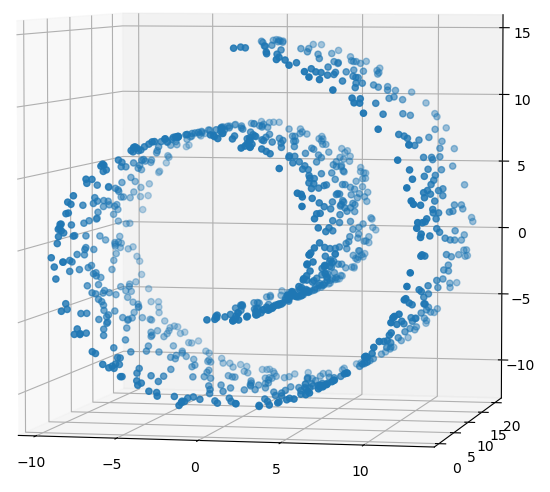
\includegraphics[height=0.4\textheight]{swiss_roll.png}
  \caption{A plot of the swiss roll dataset. We have $d=3$ but the support of the data $S$ is of dimension $r=2$}
  \label{fig:swiss_roll}
\end{figure}
  
\begin{figure}[p]
  \centering
  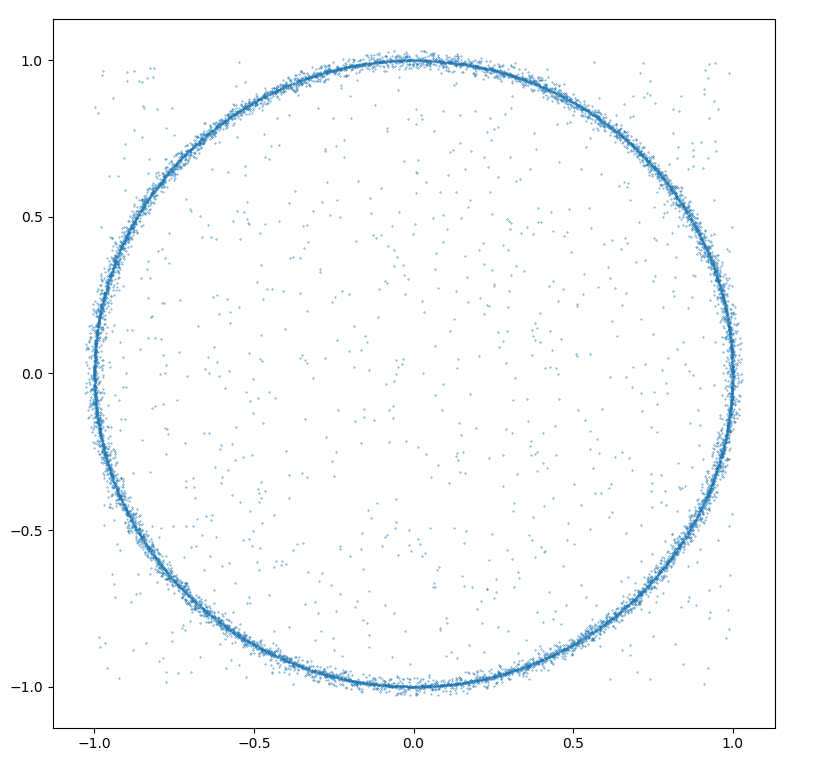
\includegraphics[height=0.4\textheight]{high_concentration.png}
  \caption{On this plot we have a dataset of dimension 2 but there is a support of dimension 1 that concentrates a big part of the mass}
  \label{fig:high_concentration}
\end{figure}

\newpage

An estimator of $S$ is $\widehat{S} = \bigcup^n_{i=1} B(X_i, \varepsilon_n)$. The estimator $\widehat{S}$ is $d$-dimensional but converges to $S$. The Hausdorff distance $H(A,B)$ between two sets $A$ and $B$ is:

\begin{center}
  $H(A,B) =$ inf$ \lbrace \varepsilon : A \subset B \oplus \varepsilon$ and $B \subset A \oplus \varepsilon \rbrace$ 
\end{center}

where 

\begin{center}
  $A \oplus \varepsilon = \bigcup\limits_{x \in A} \B(x,\varepsilon)$ 
\end{center}

with $\B(x, \varepsilon)$ the ball of radius $\varepsilon$ centered on $x$. Assume $S$ to be $r$-dimensional and $P$ to have its mass spread all over $S$. Formally: $\exists c > 0 \mid \forall x \in S, \varepsilon > 0, P(B(x, \varepsilon)) \ge c\varepsilon^r$ and the number of balls of size $\varepsilon$ required to cover $S$ is $C(\frac{1}{\varepsilon})^r$. Then:\\

  $P(H(\widehat{S},S) > 2\varepsilon)$\\
  $= P($there is no ball in $S \oplus \varepsilon$ with no sample point inside)\\
  $\le C\varepsilon^{-r} \max_k (1-P(X_1 \in B_k))^n$\\
  $\le C\varepsilon^{-r} (1-\min_k P(X_1 \in B_k))^n$\\
  $\le C\varepsilon^{-r}e^{-nc\varepsilon^r}$ (using $P(X\in B_k) \ge c\varepsilon^r$ and $(1-x)^n \le exp(-nx)$ for $0 \le x \le 1$)
\\
which converges.\\

Note that we only verify one of the two inclusions for the Hausdorff distance since the other one is always respected.\\

Now that we can find an estimation for a manifold that would concentrate all or most of a distribution. We try to estimate the topology of a manifold. That will be done in details with persistent homology however let us tackle the topic already. To estimate the topology of a set, one can try to find an estimator of the topology that is topologically similar to the studied set. Studying topological similarity comes down to the study of the existence of homeomorphism i.e. of bi-continuous maps. Markov \cite{markov_insolubility_2001} showed that in general the question is undecidable for dimension greater than four. That is why instead we determine if two sets are homologically equivalent.\\

A result in topology and statistics showed that:
\begin{center}
  $\widehat{S} = \bigcup\limits_{i=1}^{n}\B(X_i,\varepsilon)$
\end{center}

has the homology of $S$ with high probability as long as $S$ has a positive reach and $\varepsilon$ remains relatively small compared to it. The reach $r$ of a set $S$ is the largest real number such that any point within distance $r$ of $S$ has a unique projection on $S$.

\subsubsection{Persistent homology}

Persistent homology is the computationable side of homology theory. Persistent homology is the name given to an algorithm aiming to compute the topological features of data. We have discussed in detail homology from a mathematical point of view in \textbf{Section \ref{sec:homology}} and have shown that for $n \ge 2$, an $n$-dimensional sphere has for homology group: $H_n^\Delta(\S^n) \approx \Z$. To simplify vocabulary and notation we will be using betti numbers. Betti numbers of an $n$-dimensional topological space $X$ counts the ranks of the groups each $(H_k^\Delta(X))_{0 \le k \le n}$ is topologically equivalent to. In the case of the torus $T$, the betti number are $(1,2,1,0)$. Recalling the formula to compute $H_k^\Delta(X) = \frac{\text{Ker} \delta_n}{\text{Im} \delta_{n+1}}$, since $C_{n+1} = \emptyset$, $\delta_{n+1} = 0$ and hence any value $(H_k^\Delta(X))_{k > n} = 0$. Therefore, it is conventionally admitted not to write betti numbers above that value.\\

To properly define persistent homology one must first define the distance function between a set $S$ and a point $x$. It is written as:
\begin{center}
  $d_s(x) = \inf\limits_{y\in S} ||x-y||$  
\end{center}

The lower level sets of the distance function are

\begin{center}
  $L_\varepsilon = \lbrace x : d_S(x) \le \varepsilon \rbrace$
\end{center}

It is equivalent to writting:

\begin{center}
  $L_\varepsilon = \bigcup\limits_{x \in S} B(x,\varepsilon)$ 
\end{center}

As $\varepsilon$ increases, $L_\varepsilon$ changes. Different topological features (represented by the homology groups and the betti numbers) will appear and disappear. Consider $\S^1$, at first when $\varepsilon < 1$, we have the betti numbers being $(0,1,0)$ and once $\varepsilon$ reaches 1, the betti numbers become $(1,0,0)$ (cf Figure \ref{fig:betti_s1}). 

\begin{figure}[h]
  \begin{minipage}[c]{.32\linewidth}
             \centering
            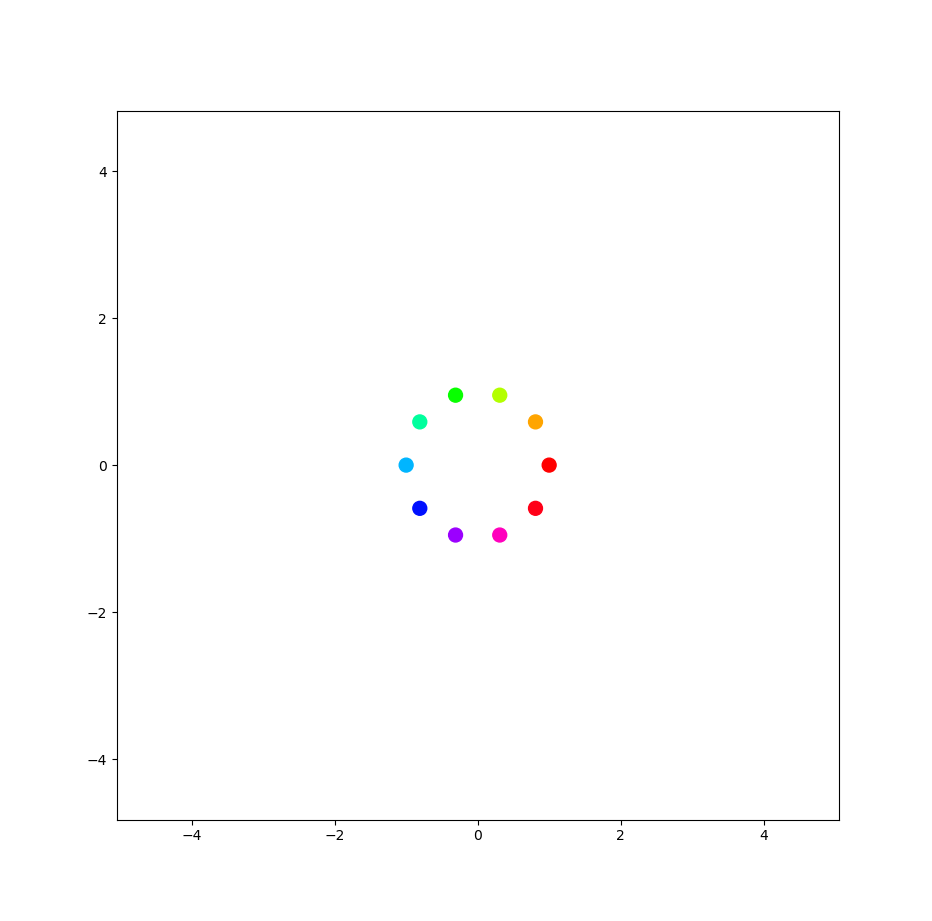
\includegraphics[width=1.0\textwidth]{circle_small_eps.png}
         \end{minipage}
         \hfill%   
         \begin{minipage}[c]{.32\linewidth}
             \centering
            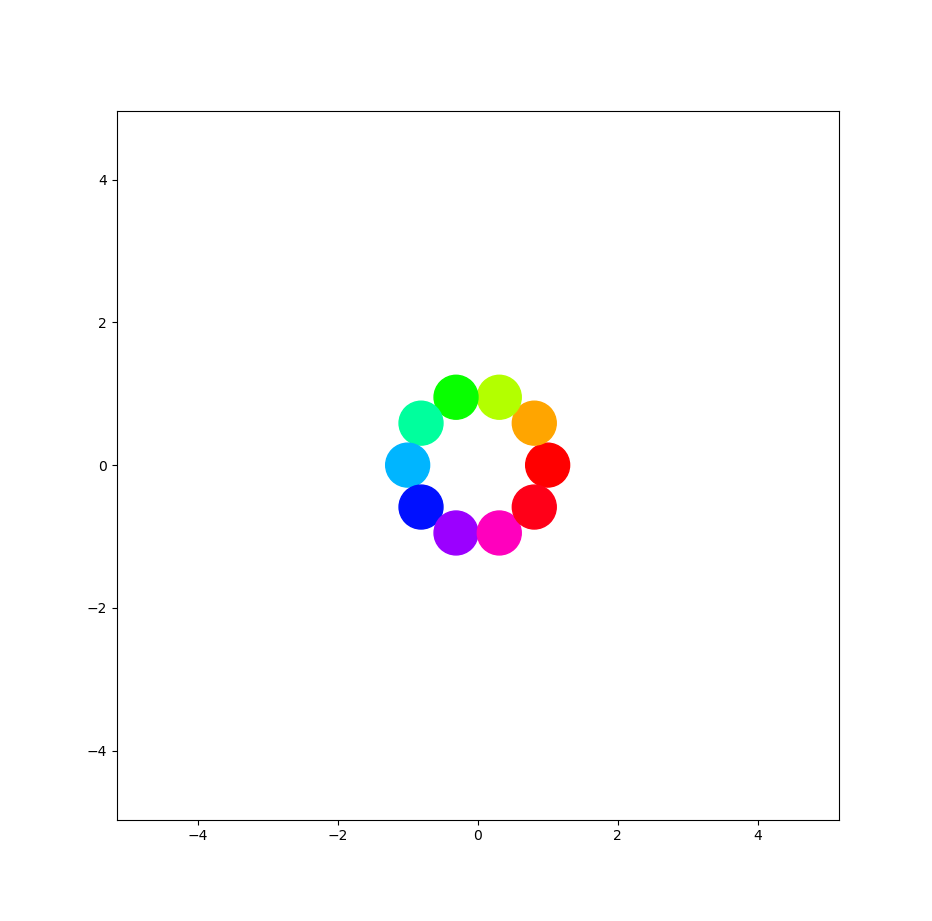
\includegraphics[width=1.0\textwidth]{circle_mid_eps.png}
        \end{minipage}
         \hfill%   
         \begin{minipage}[c]{.32\linewidth}
             \centering
            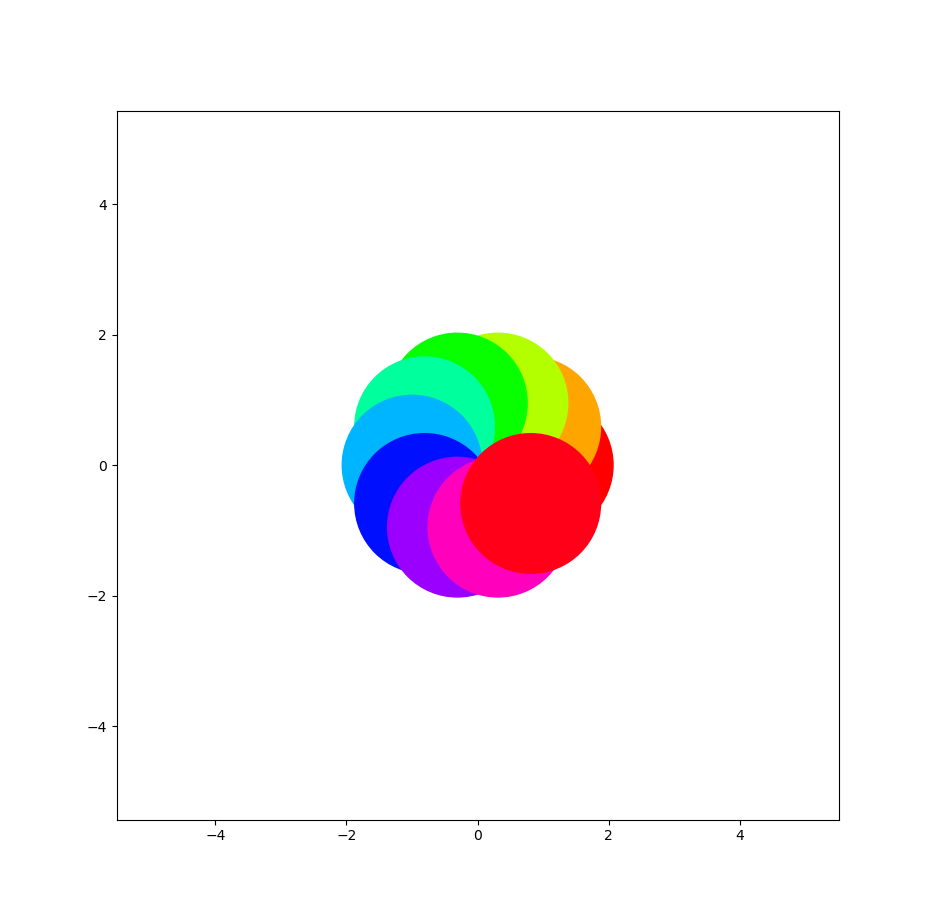
\includegraphics[width=1.0\textwidth]{circle_big_eps.png}
        \end{minipage}
        \caption{Three plots for a dataset with data on $\S^1$. The betti numbers are from left to right: $(10,0,0)$, $(0,1,0)$, $(1,0,0)$}
  \label{fig:betti_s1}
\end{figure}

Considering the evolution of $L_\varepsilon$, one can draw a persistence diagram (cf Figure \ref{fig:persistence_diagram}) and a barcode diagram (cf Figure \ref{fig:persistence_barcode}) that are equivalent. The barcode diagram represents the time of birth and death of each topological feature with a bar for each persistent generator. You will note that the full circle obtained from the merge of all balls around each point is considered to be the obtained from one of the original generator hence its big persistence. The persistence diagram represents with a point the birth and death of each topological feature, considering the symetry of our figure, there are 9 points on coordinate $\approx(0,0.1)$.\\ 

\begin{figure}[p]
             \centering
            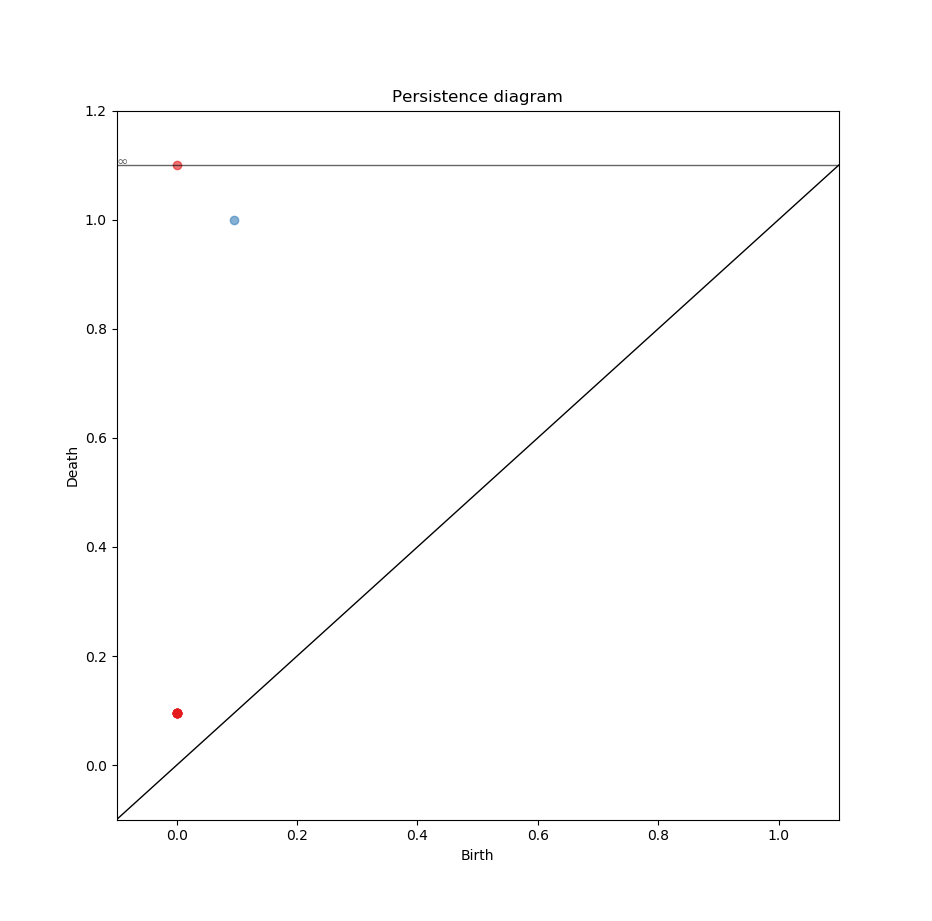
\includegraphics[height=.45\textheight]{circle_persistence_diagram.png}
        \caption{The persistence diagram of dataset from Figure \ref{fig:betti_s1}}
        \label{fig:persistence_diagram}
\end{figure}

\begin{figure}[p]
             \centering
            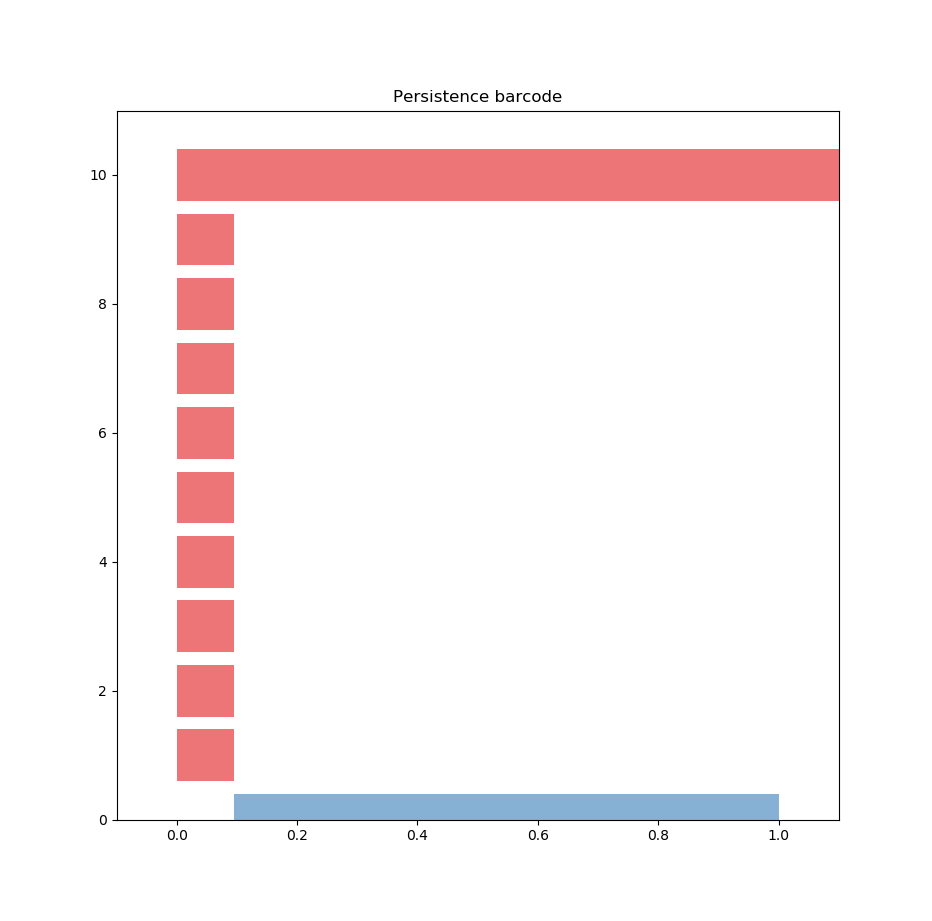
\includegraphics[width=.45\textheight]{circle_persistence_barcode.png}
        \caption{The barcode diagram of dataset from Figure \ref{fig:betti_s1}}
        \label{fig:persistence_barcode}
\end{figure}

Note that an infinite is defined on the right of the barcode and the top of the y-axis of the persistence diagram. It corresponds to the value of $\varepsilon_\infty = \max\limits_{x,y \in S} ||x-y||$. Equivalently $\forall x,y \in \S, x \in \B(y ,\varepsilon_\infty)$ and $y \in \B(x, \varepsilon_\infty)$. To the different persistence, we define the bottleneck distance. Given two persistence diagram $D_1, D_2$:

\begin{center}
  $\delta_\infty(D_1, D_2) = \inf\limits_{\gamma} \sup\limits_{z \in D_1} ||z - \gamma(z)||_\infty$
\end{center}

with $\gamma$ covering the set of bijections between $D_1$ and $D_2$. The image behind it is to overlay the two diagrams and look at how to match the points as well as possible to minimize the distance between them.\\

To compute the dimension of the structure persistent homology one uses $\Delta$-complexes by using an object called the $\check{C}$ech complex $C_\varepsilon$. It is defined as follows. All singletons are included in $C_\varepsilon$, there are $0$-dimensional simplices. All pairs of points $X_i, X_j$ such that $||X_i - X_j|| \le \varepsilon$ are included in $C_\varepsilon$, these are $1$-dimensional simplices. Each triplet $X_i, X_j, X_k$ such that $B(X_i, \varepsilon/2) \cap B(X_j, \varepsilon/2) \cap B(X_k, \varepsilon/2) \neq \emptyset$ is included, these are 2-dimensional simplices. And so on.\\ 

A more computationally efficient way to compute complexes is called the Vectoris-Rips complex $V_\epsilon$ and is defined as follows. A simplex is included in $V_\epsilon$ if each parir of vertices is no more than $\varepsilon$ apart. It can be shown that the persistent homology defined by $V_\varepsilon$ approximates the persistent homology defined by $C_\varepsilon$ .

\subsection{Knot theory}

Knot theory is a part of topology concerned with the study of mathematical knots. They are inspired by real life knots  that can be done on ropes or shoelaces but differs in the sense that the ends are joined together so that it can not be undone. There are multiple ways to describe knots and we will cover some of them. One of the key concepts of knot theory is equivalence. Two knots are considered equivalent if they can be transformed in each other without cutting the rope open. We will formalize these notions in this part relying on the class given by Pr. Anthony Bosman at Andrew University \cite{anthony_bosman_knot_2019}.

\subsubsection{Fundamental concepts}

\begin{definition}
  A knot is an embedding of a circle in 3-dimensional euclidian space $\R^3$
\end{definition}

A knot is bounded by all of its homeomorphism since we are studying it from a topological point of view. Two mathematical knots are equivalent if they are ambient isotopic (can be deformed into the other via a deformation of $\R^3$ upon itself).\\

\begin{definition}
  let $N$ and $M$ be manifolds and $g$ and $h$ be embeddings of $N$ and $M$. A continuous map:
   \begin{center}
     $F: M \times [0,1] \to M$
   \end{center}
  is defined to be an ambient isotopy taking $g$ to $h$ if $F_0$ is the identity and each map $F_t$ is an homeomorphism from $M$ to itself, and $F_1 \circ g = h$.
\end{definition}

  Knot representation might for further explained purpose be oriented giving an orientation to each of its crossings. That result with two types of crossings left-handed crossing and right-handed crossings as shown in Figure \ref{fig:oriented_knot}

\begin{figure}[H]
  \begin{minipage}[c]{.5\textwidth}
  \centering
  
\includegraphics[width=.9\textwidth]{trefoil_oriented.png}    
  \end{minipage}
  \begin{minipage}[c]{.20\textwidth}
  \centering
  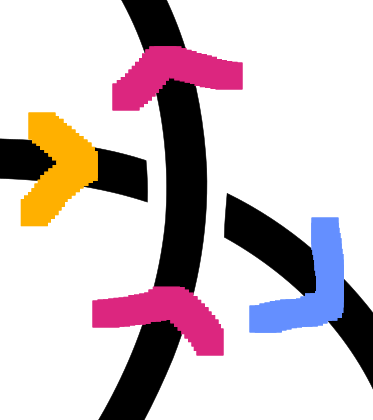
\includegraphics[width=.9\textwidth]{left_crossing.png}    
  \caption{Left-handed crossing}
  \end{minipage}
  \begin{minipage}[c]{.20\textwidth}
  \centering
  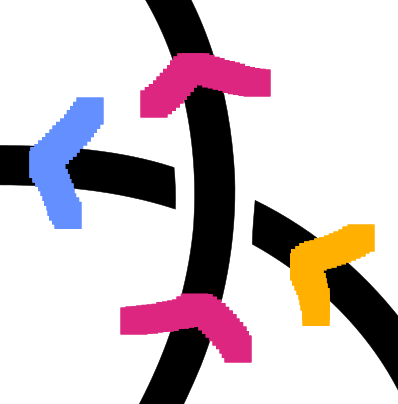
\includegraphics[width=.9\textwidth]{right_crossing.png}    
  \caption{Right-handed crossing}
  \end{minipage}
  \caption{On the left an oriented trefoil, on the right a left-handed knot and a right-handed knot}
  \label{fig:oriented_knot} 
\end{figure}

That is to say there is a map $F$ with a parameter $t$ ranging from 0 to 1, sending for $t=0$, $h$ to itself and for $t = 1$, $h$ to $g$.\\

In 1927, Reidemeister showed that ambient isotopy was equivalent to a set of three moves that can be performed on knots \cite{reidemeister_elementare_1927}. The three moves are as follow:

\begin{itemize}
    \item Type I: Twist
\begin{figure}[H]
             \centering
            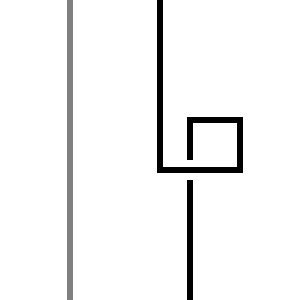
\includegraphics[height=100pt]{r1.png}
            \caption{The Reidemeister twist transformation}
        \label{fig:r_1}
\end{figure}
    \item Type II: Poke
\begin{figure}[H]
             \centering
            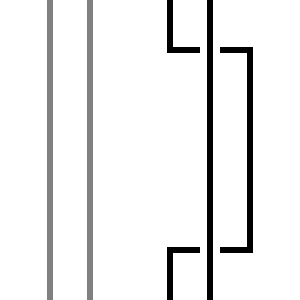
\includegraphics[height=100pt]{r2.png}
            \caption{The Reidemeister poke transformation}
        \label{fig:r_2}
\end{figure}
    \item Type III: Slide 
\begin{figure}[H]
             \centering
            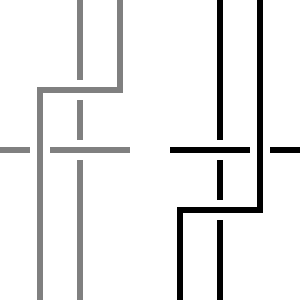
\includegraphics[height=100pt]{r3.png}
            \caption{The Reidemeister slide transformation}
        \label{fig:r_3}
\end{figure}
  \end{itemize}

i.e. two knots are equivalent if they can transformed into each others using only these three moves.\\

Knot are composed of crossings and components. The crossings are the point where the embedding overlaps itself and the components are the parts of the embedding between the crossing. We will later number the components and crossings to perform computations on knots. It is important to note that cannonically the knots are classified in category representing the minimal number of crossing that can be obtained by a representation of a knot. You can find the beginning of the knot table sorted by increasing number of crossings in Figure \ref{fig:knot_table}.

\begin{figure}[H]
  \centering
  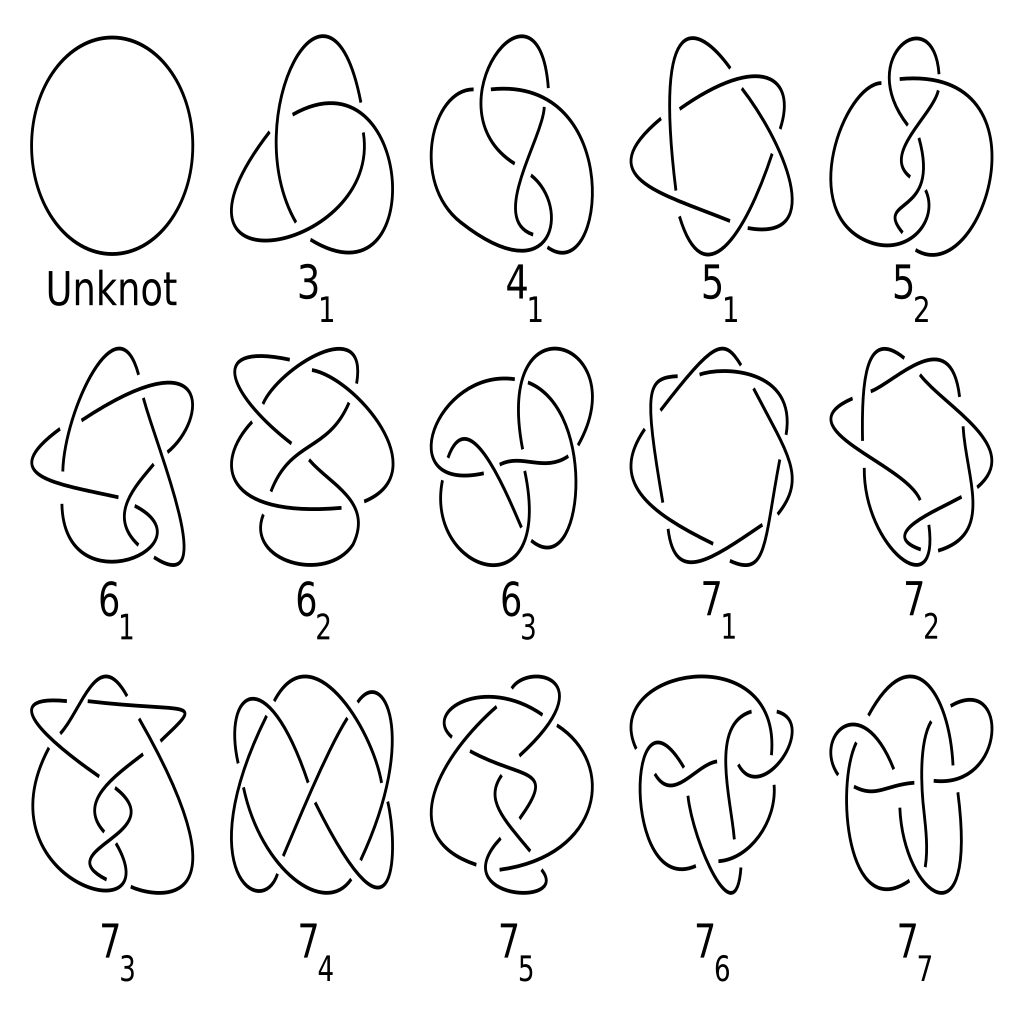
\includegraphics[width=.6\textwidth]{knot_table.png}
  \caption{Knot table up to 7 crossings knots}
  \label{fig:knot_table}
\end{figure}

\subsubsection{Knot invariants}

One of the main question of knot theory is to find a way to identify any two equivalent knots. As of today, such method is still to be found. Two knots that might seem very different can be equivalent as shown in Figure \ref{fig:unknot}. To partially solve the problem, researcher have found knot invariants, that is to say mathematical object computable from any knot representation and that will always be equal for two representation of the same knot. We will be in this section introducing some of these and explain the one we will be using for our research.\\

\begin{figure}[H]
  \begin{minipage}[c]{.2\textwidth}
  \centering
  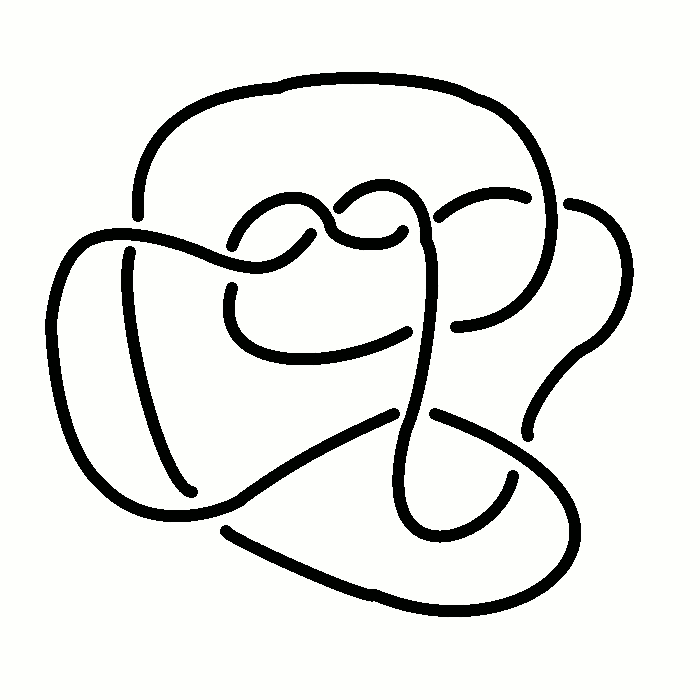
\includegraphics[width=.95\textwidth]{knot_unfolding-0.png}
    
  \end{minipage}
  \hfill
  \begin{minipage}[c]{.2\textwidth}
  \centering
  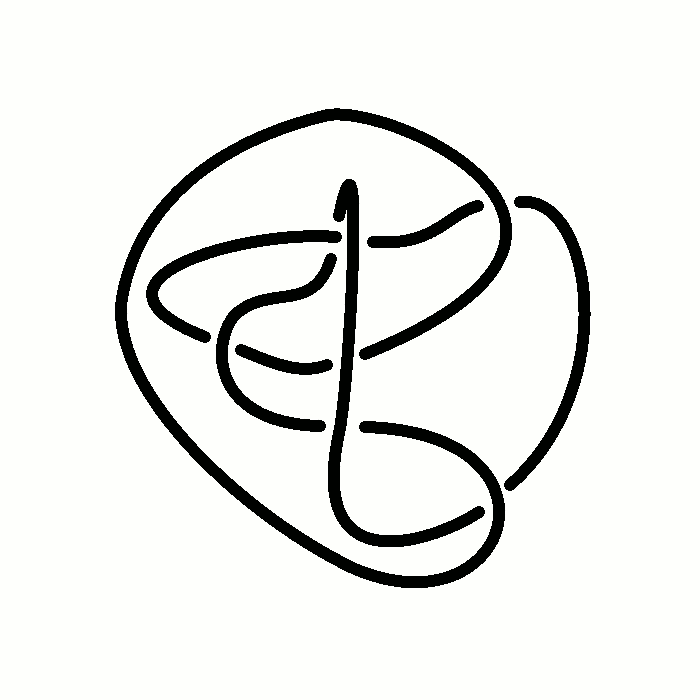
\includegraphics[width=.95\textwidth]{knot_unfolding-10.png}
    
  \end{minipage}
  \hfill
  \begin{minipage}[c]{.2\textwidth}
  \centering
  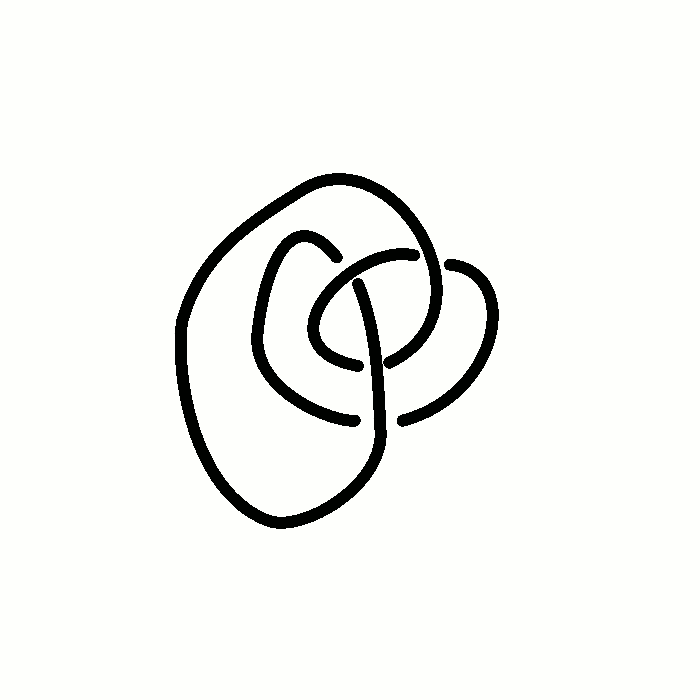
\includegraphics[width=.95\textwidth]{knot_unfolding-20.png}
    
  \end{minipage}\\
  \begin{minipage}[c]{.2\textwidth}
  \centering
  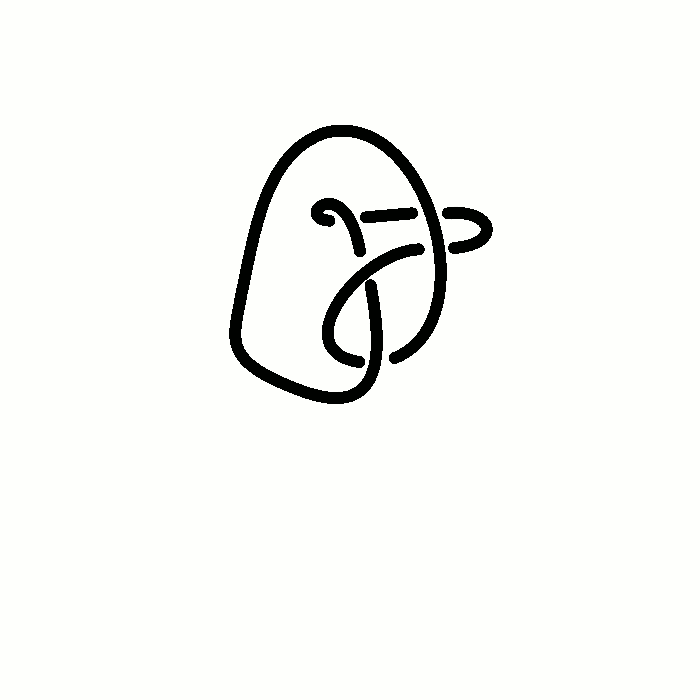
\includegraphics[width=.95\textwidth]{knot_unfolding-30.png}
    
  \end{minipage}
  \hfill
  \begin{minipage}[c]{.2\textwidth}
  \centering
  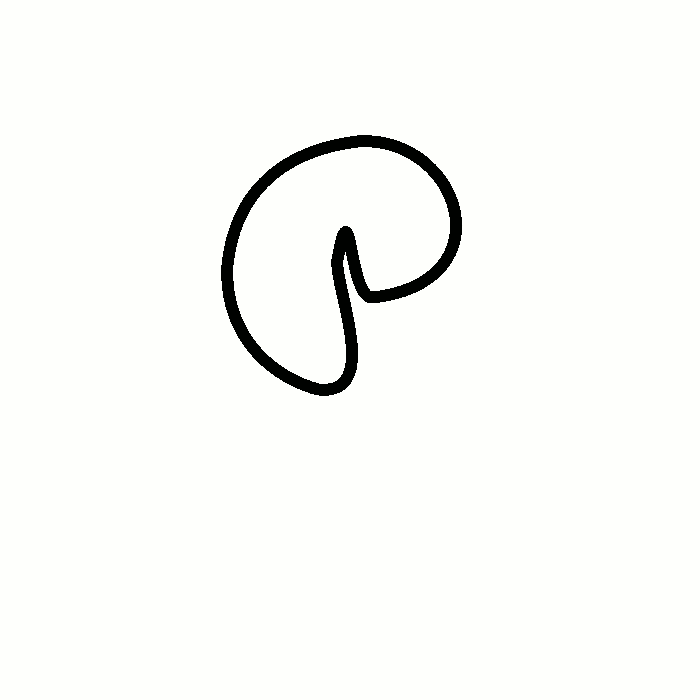
\includegraphics[width=.95\textwidth]{knot_unfolding-40.png}
    
  \end{minipage}
  \hfill
  \begin{minipage}[c]{.2\textwidth}
  \centering
  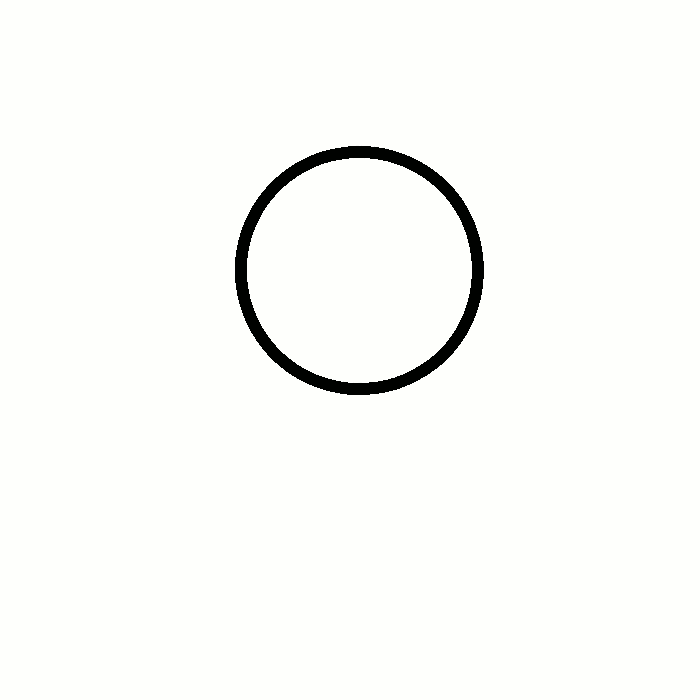
\includegraphics[width=.95\textwidth]{knot_unfolding-50.png}
    
  \end{minipage}
  \caption{Knot unfolding}
  \label{fig:unknot}
  
\end{figure}

\paragraph{Tricolorability (or 3-colorability)}

Tricolorability is a criterion to color the components of a knot following two rules:

\begin{itemize}
  \item All components must be colored
  \item At each crossing all three components are either all of the same color either all of different colors ($\Longleftrightarrow$ one can find only one or the three colors at each crossing). 
\end{itemize}

For instance the trefoil is 3-colorable as shown is Figure \ref{fig:trefoil_color} unlike the figure-eight knot (Figure \ref{fig:figure8})\\


\begin{figure}[H]
  \begin{minipage}[c]{.4\textwidth}
    \centering
    
\includegraphics[width=.80\textwidth]{trefoil_color.png}
    \caption{Colored trefoil}
    \label{fig:trefoil_color}
  \end{minipage}
  \hfill
  \begin{minipage}[c]{.4\textwidth}
    \centering
    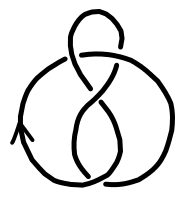
\includegraphics[width=.80\textwidth]{fig_eight_only_nat.png}
    \caption{Not-colored figure-eight knot}
    \label{fig:figure8}
  \end{minipage}  
\end{figure}

\begin{proposition}
  Tricolorabitily is a knot invariant
\end{proposition}

\begin{proof}

To prove that 3-colorability is a knot invariant it is sufficient to show that the tricolorability of a knot is preserved with the Reidemeister moves. This task is fairly simple though it might involve to test a lot of cases.

\begin{itemize}
  \item Type I: Twist. This move is straight forward since starting with only one component, the only starting point is of having a single color, the solution of keeping the same color is obvious.
\begin{figure}[H]
             \centering
            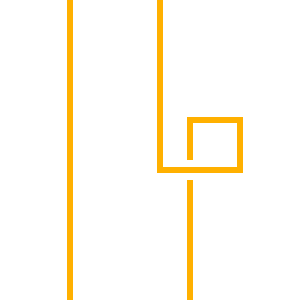
\includegraphics[height=100pt]{r1_colored.png}
          \caption{Twist tricolorability}
        \label{fig:r_1_colored}
\end{figure}

\item Type II: Poke. For this move there are two possible configuration as starter since both components can have the same color or a different one. In both case it is possible to find a coloration that fits.

\begin{figure}[H]
  \begin{minipage}[c]{.5\textwidth}
             \centering
            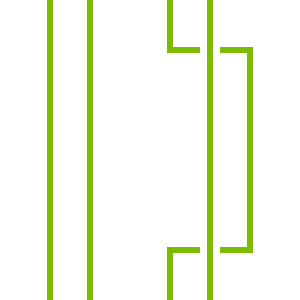
\includegraphics[height=100pt]{r2_colored_2.png}
    
  \end{minipage}
  \begin{minipage}[c]{.5\textwidth}
             \centering
            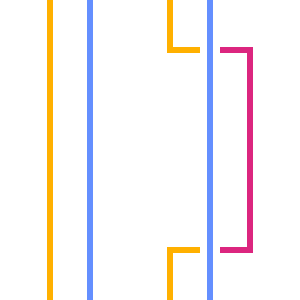
\includegraphics[height=100pt]{r2_colored.png}
    
  \end{minipage}
          \caption{Poke tricolorability}
        \label{fig:r_2_colored}
\end{figure}

\item Type III: Slide. This move could have up to 8 possibilities but the possibilities where exactly one of the crossings is of different colors is not possible since it goes against the rules of tricolorability. We end up with 5 cases that all admit a solution.   

\begin{figure}[H]
  \begin{minipage}[c]{.3\textwidth}
             \centering
            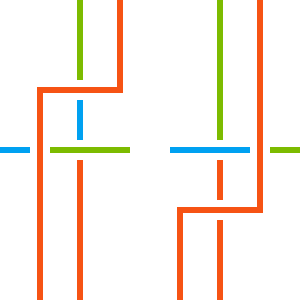
\includegraphics[height=100pt]{r3_colored_2.png}
    
  \end{minipage}
  \begin{minipage}[c]{.3\textwidth}
             \centering
            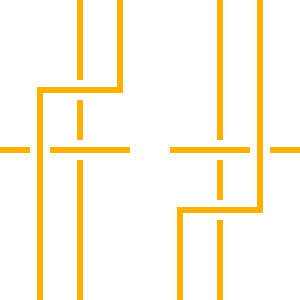
\includegraphics[height=100pt]{r3_colored.png}
    
  \end{minipage}
  \begin{minipage}[c]{.3\textwidth}
             \centering
            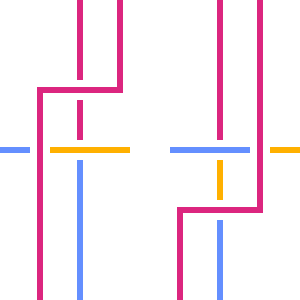
\includegraphics[height=100pt]{r3_colored_3.png}
    
  \end{minipage}
  \begin{minipage}[c]{.5\textwidth}
             \centering
            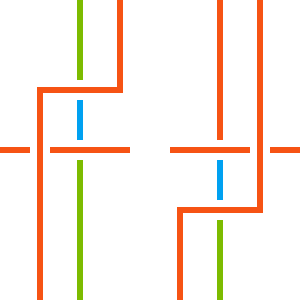
\includegraphics[height=100pt]{r3_colored_4.png}
    
  \end{minipage}
  \begin{minipage}[c]{.5\textwidth}
             \centering
            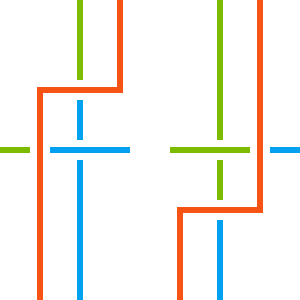
\includegraphics[height=100pt]{r3_colored_5.png}
    
  \end{minipage}
          \caption{Slide tricolorability}
        \label{fig:r_3_colored}
\end{figure}
\end{itemize}

Note that a solution is admissible only if the components that link with the rest of the knot can preserve their color so that the move do not interfere with the rest of the knot.

\end{proof}

Tricolorability is a useful invariant because it can allow for example to prove that the trefoil ($3_1$) and the figure-eight knot ($4_1$) or different knots, however it does not allow to discriminate a lot of knots since for example with tricolorability only, there is no way to know wether the unknot is different from the figure-eight knot. In Figure \ref{fig:tricolor_table} we see which knots are tricolorable. To be able to discriminate more knots we will introduce another tool, the knot determinant. 

\begin{figure}[H]
  \centering
  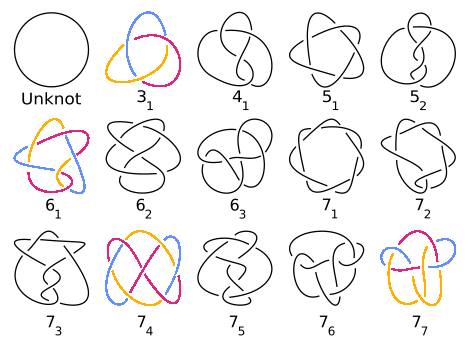
\includegraphics[width=.6\textwidth]{tricolorability_table.png}
  \caption{Tricolorability table}
  \label{fig:tricolor_table}
\end{figure}

\paragraph{Knot determinant}
\label{sec:knot_det}

To be able to compute knot determinant, one must first number components and crossings of a knot as shown in Figure \ref{fig:trefoil_number}.

\begin{figure}[H]
  \centering
  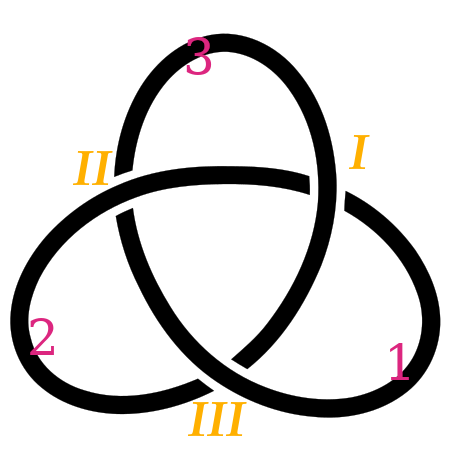
\includegraphics[width=.6\textwidth]{trefoil_number.png}
  \caption{Trefoil with numbering to compute determinant}
  \label{fig:trefoil_number}
\end{figure}

One can then create a matrix $A$ with coefficient $a_{i}{j}$ defined as follows:\\

\begin{center}
  $a_{i,j} =
  \begin{cases}
    -1 &\text{if component $i$ is one of the lower components involved in crossing $j$}\\
    2 &\text{if component $i$ is the upper component involved in crossing $j$}\\
    0 &\text{otherwise}
  \end{cases}$
\end{center}

For the trefoil in Figure \ref{fig:trefoil_number} we have:

\begin{center}
$
  A = \kbordermatrix{
    & I & II & III \\
    1 & -1 & -1 & 2  \\
    2 & -1 & 2 & -1  \\
    3 & 2 & -1 & -1  \\
  }
$
\end{center}

The knot determinant is then the determinant of the matrix $A$ with one line and column removed. In the case of the previously obtained matrix, 3.\\

In the same fashion as the proof done for tricolorability one can show that the determinant is a knot invariant by showing its invariability under the Reidemeister moves.\\

The results of the computation of knot determinants for the knots up to 7 crossings can be seen in Table \ref{tab:knot_determinant}.

\begin{table}[H]
\begin{center}
  \begin{tabular}{| c | c |}
    \hline
    knot & $det(K)$\\
    \hline
    $3_1$ & 3\\
    \hline
    $4_1$ & 5\\
    \hline
    $5_1$ & 5\\
    \hline
    $5_2$ & 7\\
    \hline
    $6_1$ & 9\\
    \hline
    $6_2$ & 11\\
    \hline
    $6_3$ & 13\\
    \hline
    $7_1$ & 7\\
    \hline
    $7_2$ & 11\\
    \hline
    $7_3$ & 13\\
    \hline
    $7_4$ & 15\\
    \hline
    $7_5$ & 17\\
    \hline
    $7_6$ & 19\\
    \hline
    $7_7$ & 21\\
    \hline
  \end{tabular}
\end{center}
  \caption{Knot table \& determinant}
\label{tab:knot_determinant}
\end{table}

We can see that even though more values are possible it can not allow to discriminate all knots.\\

Note that the result obtained from the computation of the knot determinant gives the $p$-colorability of a knot. Extending the concept of $3$-coloration by keeping the same rules (1 or 3 colors at each crossing), we notice that a $p$-coloration is possible iff $p$ is a divisor of the knot determinant.

\paragraph{Alexander polynomial}

The last knot invariant that we will introduce in this paper is the Alexander polynomial. Its definition is close to the one of the determinant. To compute the Alexander polynomial, one will first construct a matrix $A$ with coefficients $a_{i,j}$ defined as such: 

\begin{center}
  $a_{i,j} =
  \begin{cases}
    t &\text{if component $i$ \textcolor{blue}{enters} \textcolor{red}{exists} under \textcolor{blue}{left} \textcolor{red}{right} handed crossing $j$}\\
    -1 &\text{if component $i$ \textcolor{red}{exits} \textcolor{blue}{enters} under \textcolor{red}{left} \textcolor{blue}{right} handed crossing $j$}\\
    1-t &\text{if component $i$ is overcrossing at crossing $j$}\\
    0 &\text{otherwise}
  \end{cases}$
\end{center}

\begin{figure}[H]
  \begin{minipage}[c]{.50\textwidth}
  \centering
  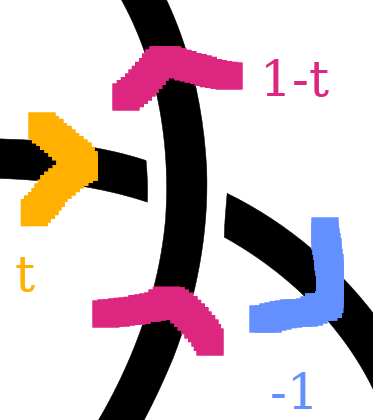
\includegraphics[width=.3\textwidth]{left_crossing_number.png}    
  \caption{Left crossing}
  \end{minipage}
  \hfill
  \begin{minipage}[c]{.50\textwidth}
  \centering
  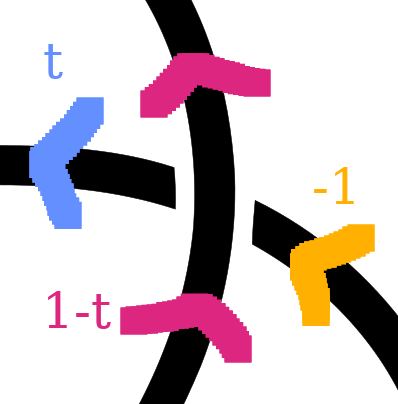
\includegraphics[width=.3\textwidth]{right_crossing_number.png}    
  \caption{Right crossing}
  \end{minipage}
  \label{fig:oriented_knot_alexander} 
\end{figure}

Then in the same manner, one can compute the determinant after removing one line and column of the matrix. For the trefoil we obtain:\\

\begin{center}
$
  A = \kbordermatrix{
    & I & II & III \\
    1 & -1 & t & 1-t  \\
    2 & t & 1-t & -1  \\
    3 & 1-t & -1 & t  \\
  }
$
\end{center}

After normalization, we obtain the polynomial: $t - 1 + t^{-1}$. The polynomial obtained by this method can differ from a factor $\pm t^n, n \in \N$. To solve that issue we normalize it so that it looks symetric (Laurent polynomial) and denote if $\Delta_k(t)$. We can with that method write a table of the Alexander polynomial as seen in Table \ref{tab:knot_alexander} for the knots up to 7 crossings.

\begin{table}[H]
\begin{center}
  \begin{tabular}{| c | c |}
    \hline
    knot & $\Delta_k(t)$\\
    \hline
    $3_1$ & $t - 1 + t^{-1}$\\
    \hline
    $4_1$ & $-t + 3 -t^{-1}$\\
    \hline
    $5_1$ & $t^2 - t + t - t^{-1} + t^{-2}$\\
    \hline
    $5_2$ & $2t - 3 + 2t^{-1}$\\
    \hline
    $6_1$ & $-2t + 5 -2t^{-1}$\\
    \hline
    $6_2$ & $-t^2 + 3t -3 + 3t^{-1} - t^{-2}$\\
    \hline
    $6_3$ & $t^2 - 3t +5 -3t^{-1} + t^{-2}$\\
    \hline
    $7_1$ & $t^3 - t^2 +t -1 + t^{-1} - t^{-2} + t^{-3}$\\
    \hline
    $7_2$ & $3t -5 + 3t^{-1}$\\
    \hline
    $7_3$ & $2t^2 - 3t + 3 - 3t^{-1} + 2t^{-2}$\\
    \hline
    $7_4$ & $4t -7 + 4t^{-1}$\\
    \hline
    $7_5$ & $2t^2 - 4t + 5 - 4t^{-1} + 2t^{-2}$\\
    \hline
    $7_6$ & $-t^2 +5t -7 +5t^{-1} - t^{-2}$\\
    \hline
    $7_7$ & $t^2 -5t +9 -5t^{-1} + t^{-2}$\\
    \hline
  \end{tabular}
\end{center}
  \caption{Knot table and Alexander polynomial}
\label{tab:knot_alexander}
\end{table}

With the Alexander polynomial one can discrimainate any two knots with up to seven crossings. Though the Alexander polynomial can not discriminate any to knots as explained in the introduction. An interesting property of the Alexander polynomial is that $\Delta_k(-1) = det(K)$ (the knot determinant).

\newpage
\thispagestyle{empty}
\mbox{}
\newpage

\section{Previous research on quantification of neural network expressiveness}

In this section we will explain how the topic of quantifying neural network expressiveness has been tackled by researchers and introduce the different research articles on which our work relies.\\

The concept of measuring neural network expressiveness induces to use some concept as a measure of difficulty of expression. In this section we will see how some previously introduced concepts can be used as measures: betti numbers and circle embeddings. 

\subsection{Using topological data analysis}

\label{sec:tda_bib}

In this section we will focus on the use of betti as a measure for neural netwok expresiveness.\\

In \cite{bianchini_complexity_2014}, Bianchini and Scarselli have offered proofs on the number of neurons required in different architecture of neural network to properly express a dataset betti numbers. They have worked on determining upper bounds and lower bounds on the number of neurons required in network of a certain depth to be able to express the homology represented by its sum of betti numbers with different activation functions. Their result are summed up in Table \ref{tab:betti_up_low_bound} that can also be found in \cite{bianchini_complexity_2014}.\\

Let $X$ be a topological space. We denote $\B(X) = \sum\limits_{i} \B_i(X)$ where $\B_i(X)$ is the number of $i$-dimensional homology in $X$.

\begin{table}[H]
  \begin{center}
    \begin{tabular}{| l | l | l | c |}
      \hline
Inputs                  & \multicolumn{1}{c|}{Layers} & \multicolumn{1}{c|}{Activation function} & \multicolumn{1}{c|}{Bound} \\
      \hline
\multicolumn{4}{|c|}{Upper Bounds}                            \\
      \hline
n      & 3      & threshold           & $O(h^n)$            \\
      \hline
n      & 3      & arctan           & $O((n+h)^{n+2})$            \\
      \hline
n      & 3      & polynomial of degree $r$           & $\frac{1}{2}(2+r)(1+r)^{n-1}$            \\
      \hline
1      & 3      & arctan           & $h$            \\
      \hline
n      & any    & arctan           & $2^{h(2h-1)}O((nl+n)^{n+2h})$            \\
      \hline
n      & any    & tanh           & $2^{(h(h-1))/2}O((nl+n)^{n+h})$            \\
      \hline
n      & any      & polynomial of degree $r$           & $\frac{1}{2}(2+r^l)(1+r^l)^{n-1}$            \\
      \hline
\multicolumn{4}{|c|}{Lower bounds}                            \\
      \hline
n      & 3      & any sigmoid         & $(\frac{h-1}{n})^n$\\
      \hline
n      & any & any sigmoid         & $2^{l-1}$ \\
      \hline
n      & any      & polynomial of degree $r \ge 2$    & $2^{l-1}$\\
      \hline
\end{tabular}
  \end{center}
  
  \caption{Upper bounds and lowers bounds on the growth of $\B(X)$ for networks with $h$ neurons, $n$ input and $l$ hidden layers}
  \label{tab:betti_up_low_bound}
\end{table}

To prove these bounds they use the function sum representation of neural networks as introduced in \textbf{Section \ref{sec:nn_express}} as well as classical function analysis inequalities.\\

In \cite{guss_characterizing_2018}, Guss and Salakhutdinov relying on \cite{bianchini_complexity_2014} proposed a statistical approach to the problem of giving a value to the way each Betti numbers would affect the topological expressivity of the neural network since \cite{bianchini_complexity_2014} only relies on the sum $\B(X)$.\\

To study the difficulty of learning homologically complex data, they considered fully-connected ReLU neural networks of depth $d \in [1 ... 6]$ and width $h_l = \beta_0(X)$ when $1 \le l \le d$ and $h_l \in [1 ... 500]$ when $l = 0$. It sums up with a first layer of variable width (up to 500) and the other layers width being fixed at the number of connected components (0-homology) of $X$. These networks would then be trained using standard cross-entropy loss with Adam optimizer, a fixed learning rate of 0.01 and an increasing batch size schedule.\\

They used datasets composed of two classes of 5000 points one of randomly distributed points the other one of mixtures of the uniform distribution on $\S^1$ and $\B^2$. They limited their study to $n=2$. They studied the output for datasets continuously ranging from $H(X) = \{\Z^1, 0\}$ to $H(X) = \{\Z^{30}, \Z^{30}\}$. They trained 100 of the previously described networks on each dataset and compiled the results in Figure \ref{fig:guss_results}.


In Figure \ref{fig:guss_results} we can see two distincts parts. The upper part refers to the characterization of $H_0(X)$. Each of the four plots is representing the probability of expressing $H_0(X)$ depending on $\B_0(X)$ and the number of hidden units on the fist layer of the network (the other layers having a number of hidden units fixed to $B_0(X)$). On these plots the number of hidden units ranges from $0$ to $14$ and $\B_0(X)$ from $3$ to $15$.\\

The second plot presents the same results for the proper characterization of $\B_1(X)$ with this time $\B_1(X) \in \{1,2\}$ and hidden units ranging from $0$ to 14.\\

We can see some clear tendency (that would be expected) that expression of $H_n(X)$ is improving with the reduction of $\B_n(X)$, and the increase of $l$ and $d$. The interest of such result lies in the fact of giving a possible approximation of the evolution of the probability depending on each of these parameters.\\

Unfortunately the authors did not provide the full results and code of their research and did not answer my requests to obtain them.

\begin{figure}[H]
  \centering
  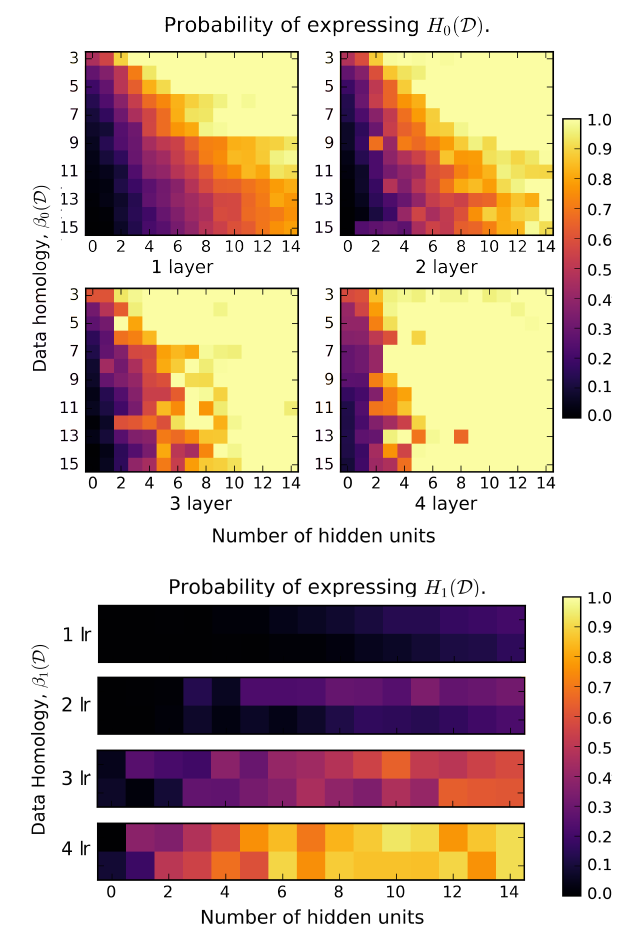
\includegraphics[width=\textwidth]{guss_res.png}
  \caption{Results on the characterization of homologies with different neural networks architecture}
  \label{fig:guss_results}
  
\end{figure}
\newpage
\subsection{Using trajectories}
\label{sec:using_trajectories}

The idea of studying trajectories to evaluate neural network expressivity comes from \cite{raghu_expressive_2017} itself relying on \cite{poole_exponential_2016} and \cite{pascanu_number_2014}.\\

In \cite{raghu_expressive_2017}, Raghu introduces various variables of interest for neural network expressivity relying on the notion of transition of activation patterns. Activation patters denotes all the way threshold-based activation functions such as ReLU and hard-tanh can activate or not at the same time. For a ReLU function we would consider it active if in the non-constant part and non-active if in the constant part. Activation patterns is a concept at network scale to summarize the existence of inputs and activation function parameters leading to different activation and non-activation of each neuron of the network.\\

To study transition Raghu introduces the unifying concept of trajectories. Trajectories are defined as follows:

\begin{definition}
  Given two points $x_0, x_1 \in \R^n$, $x(t)$ between $x_0$ and $x_1$ is a trajectory if there exists $f: [0,1] \to \R^n$ with $f(0) = 0_{\R^n}$ and $f(1) = 1_{\R^n}$ such that $x(t) = (x_0-x_1)f(t) + x_0$. 
  \label{def:trajectories}
\end{definition}

This can include simple examples such as a line with $f(t) = t$ or a circular arc with $f(t) = sin(\frac{\pi t}{2})$ but in general $x(t)$ might be more complicated. This definition is obviously linked to the concept of path in topology and therefore includes loops.\\

For piecewise linear activation functions such as ReLU and hard tanh, the function computed by the network is also piecewise linear since the linear sum of composition of piecewise linear functions is itself piecewise linear.

\begin{definition}
  We say a neuron with piecewise linear activation function transitions between input $x$ and $x+\delta$ if its activation function switches between $x$ and $x+\delta$
\end{definition}

With all the previously introduced concepts we can now give a proper definition to the activation pattern:

\begin{definition}
  The activation pattern $AP(F_A(x,W))$ of network with weights $W$, architecture $A$ and input $x$ is a string of form $\{0,1\}^{\text{number of neurons}}$ for ReLU networks and $\{-1,0,1\}^{\text{number of neurons}}$ for hard tanh networks coding the linear region of the activation function of every neuron.
\end{definition}

We can aswell define $T(F_A(x(t),W))$ the number of transition undergone by the network when $x$ sweept along $x(t)$.\\

In \cite{pascanu_number_2014}, Montufar et al. provide a bound on the number of transition by constructing a set of weights $W_0$ resulting in an exponential increase of the number of transition with the depth of the network i.e.\\

\begin{center}
  $\forall W,$ $T(F_{A_1}([0,1],W)) < T(F_{A_1}([0,1],W_0))$  
\end{center}

with $A_1$ a fully connected network with one hidden layer.\\

We denote $U(n,k,m)$ the upper bound on the number of activation patterns for a fully connected network with $n$ hidden layers of width $k$ and inputs in $\R^m$. Raghu shows that for a ReLU network we have $U(n,k,m) = O(k^{nm})$ and for hard tanh $U(n,k,m) = O((2k)^{nm})$.\\

Going back to the definition of trajectory, we define the trajectory length:

\begin{definition}
  For a trajectory $x(t)$, we define $l(x(t))$ its length to be the standard arc length:
  \begin{center}
    $l(x(t)) = \int_t \lVert \frac{dx(t)}{dt} \rVert$
  \end{center}
 
\end{definition}

Raghu then show that length grows exponentially with length in most cases. Formally:\\

\begin{theorem}
  Let $F_A(x,W)$ be a ReLU or hard tanh random neural network and $x(t)$ a one-dimensional trajectory with $x(t + \delta)$ having a non trivial perpendicular component to $x(t)$ for all $t,\delta$. Then with $z^{(d)}(x(t)) = z^{(d)}(t)$ the image of the trajectory in layer $d$ of the network we have:
  \begin{center}
    $\mathbb{E}[l(z^{(d)}(t))] \ge O(\frac{\sigma_w \sqrt{k}}{\sqrt{k+1}})^d l(x(t))$ for ReLU networks\\
    $\mathbb{E}[l(z^{(d)}(t))] \ge O(\frac{\sigma_w \sqrt{k}}{\sqrt{\sigma_w^2 + \sigma_b^2 + k\sqrt{\sigma_w^2 + \sigma_b^2}}})^d l(x(t))$ for hard tanh
  \end{center}
  with $\sigma_w$ the standard deviation of weights, $\sigma_b$ the standard deviation of bias and $k$ the width of the network.
\end{theorem}

Therefore, the length of the trajectory grows exponentially with depth and hence expressivity. A figure of that growth can be seen in Figure \ref{fig:traj_growth}.

\begin{figure}[H]
  \centering
  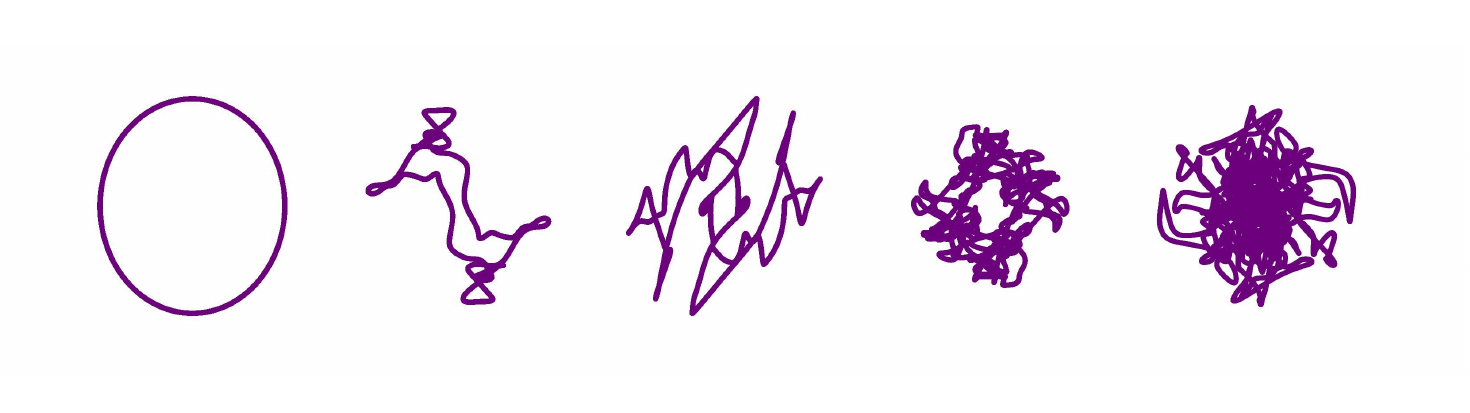
\includegraphics[width=\textwidth]{traj_growth.png}
  \caption{Projected circular trajectory at increasing layers in a width 100 neural network}
  \label{fig:traj_growth}
\end{figure}

\newpage
\thispagestyle{empty}
\mbox{}
\newpage

\section{Studying trajectories from a knot theory perspective}

In this section we will detail the work on trajectories inspired by the research detailed in \textbf{Section \ref{sec:using_trajectories}} where we study the trajectories previously introduces from a knot theory point of view.

\subsection{Methodology}

For the purpose of studying trajectories as knot we limit the definition of trajectories to the case where the beginning point is the end point ($x_0 = x_1$ in \textbf{Definition \ref{def:trajectories}}). In that case the trajectory becomes an embedding of the circle. We also limit our study to embeddings of $S^1$ in $\R^n, n \ge 3$ to ensure the existence of the knot.\\ 

Knots can exist in dimension higher than $3$ by simply living in a 3-dimensional hyperplane. We create trajectories corresponding to the first knots in increasing number of crossings namely: the unknot, the trefoil $3_1$ and the figure-eight knot $4_1$.\\

Computationnaly trajectories are arrays of points uniformly distributed along the studied embedding. They are obtained from a B-spline of hand-picked points for each different trajectory.\\

\begin{definition}
  A spline of order $n$ is a piecewise polynomial function of degree $n-1$. The values where the polynomial pieces meet are called knots and denoting them $t_0,t_1, ... , t_n$. When the knots are distincts the $n-2$ derivatives of the polynomials are continuous across each knot. When $r$ knots are coincident, only the first $n-r-1$ derivatives are continuous.
\end{definition}

For some $t_0, t_1, ... , t_n$ there is up to a scaling factor a unique spline $B_{i,n}(x)$ such that

\begin{center}
  $B_{i,n} = 
  \begin{cases}
    0 &\text{if $x < t_i$ or $x \ge t_{i+n}$}\\
    \text{nonzero} & \text{otherwise}
  \end{cases}$
\end{center}

Adding the constraint $\sum\limits_i B_{i,n}(x) = 1$ for all $x$ between the first and last knot, then we obtain unicity and $B_{i,n}(x)$ is called B-spline. Figuratively B-spline allow to create a smooth curve passing through a set of different points (knots). When some points of a B-spline repeats the smoothness is lost at those points. That last property will be important since embeddings of the circle admit the same first and last point and its B-spline representation the same first and last knot. Figure \ref{fig:knot_bspline} shows the B-spline for the trefoil and the figure-eight knot. 

\begin{figure}[H]
  \begin{minipage}[c]{.5\linewidth}
             \centering
            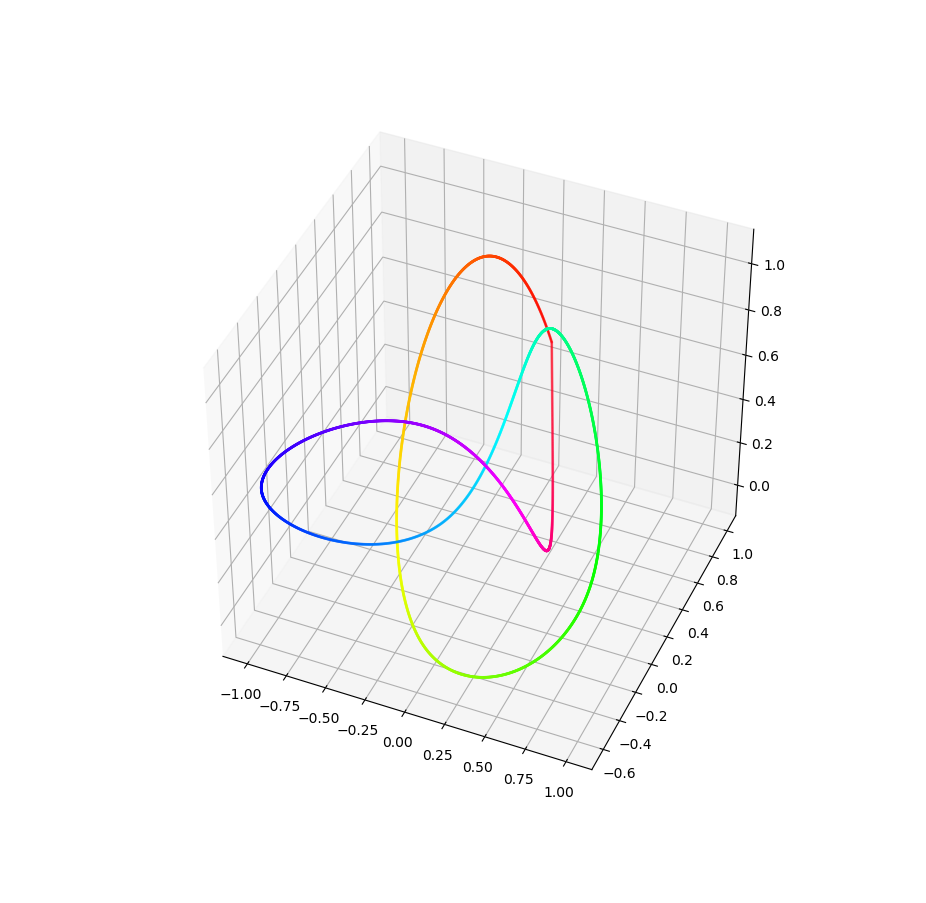
\includegraphics[width=1.0\textwidth]{trefoil.png}
         \end{minipage}
         \hfill%   
         \begin{minipage}[c]{.5\linewidth}
             \centering
             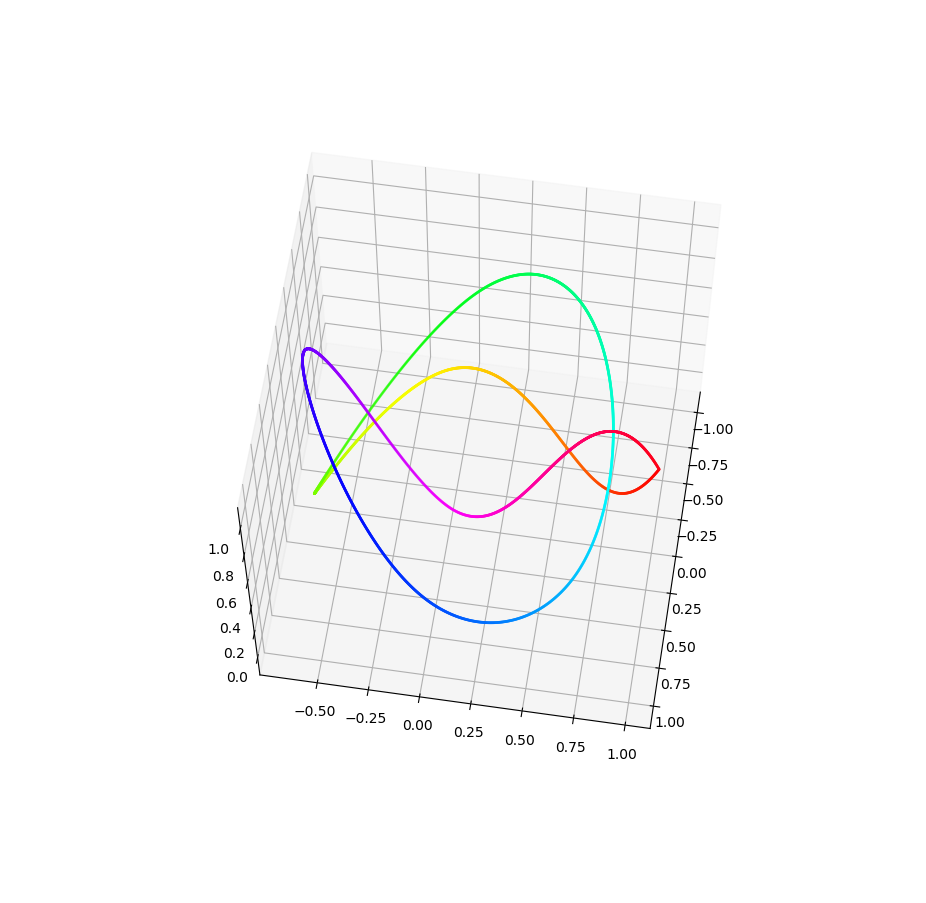
\includegraphics[width=1.0\textwidth]{figure_eight.png}
        \end{minipage}
        \caption{B-spline for $3_1$ and $4_1$ in $\R^3$}
        \label{fig:knot_bspline}
\end{figure}

The points used to generate the B-spline of $3_1$ and $4_1$ in $\R^3$ are represented in Figure \ref{fig:bspline_points}

\begin{figure}[H]
  \begin{minipage}[c]{.5\linewidth}
             \centering
            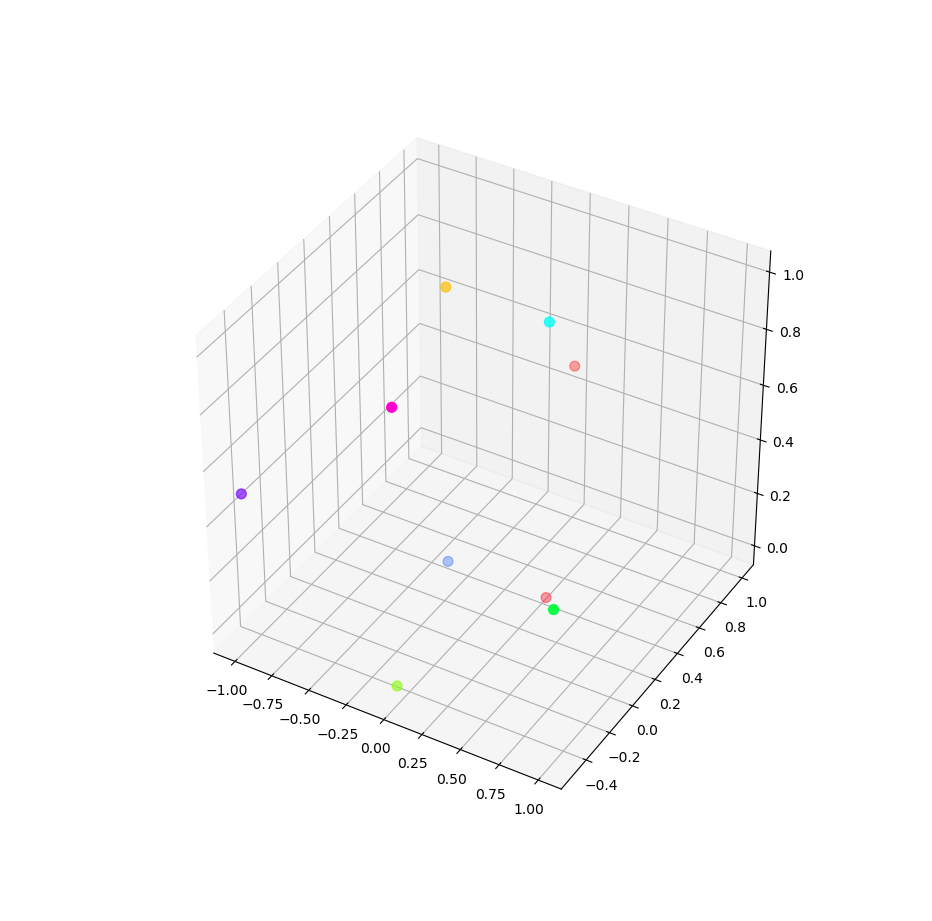
\includegraphics[width=1.0\textwidth]{trefoil_points.png}
         \end{minipage}
         \hfill%   
         \begin{minipage}[c]{.5\linewidth}
             \centering
             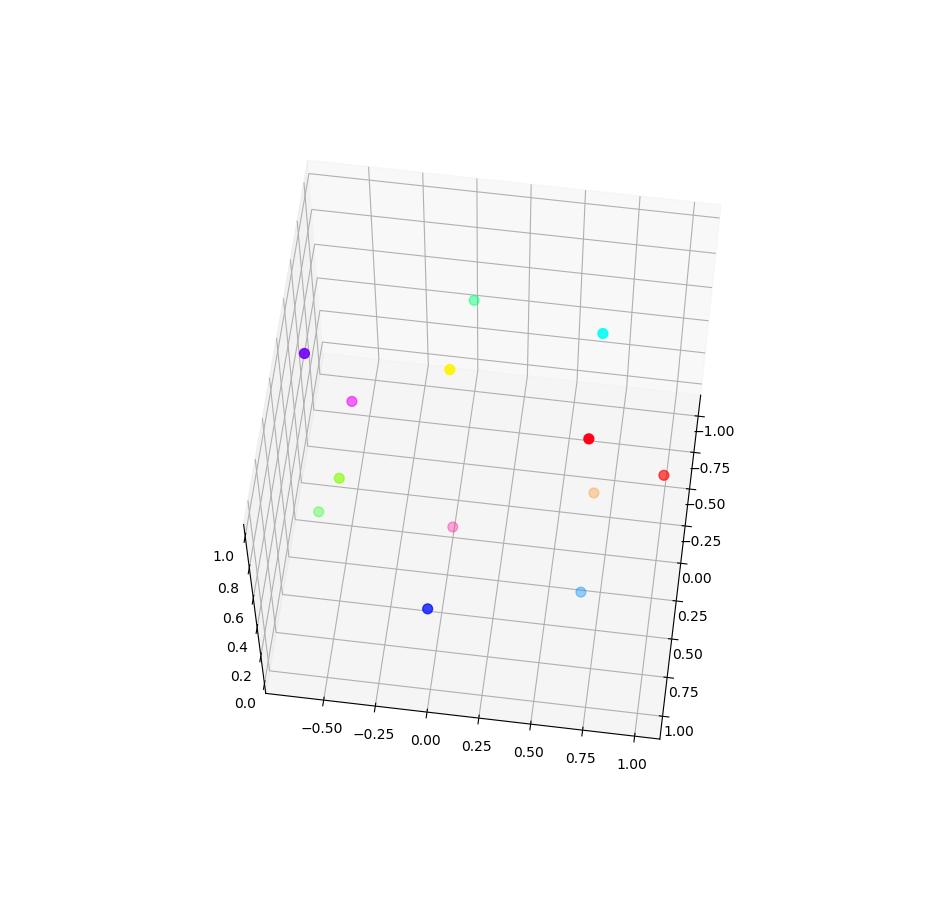
\includegraphics[width=1.0\textwidth]{fig8_points.png}
        \end{minipage}
        \caption{Points for the computation of the B-spline of $3_1$ and $4_1$ in $\R^3$}
        \label{fig:bspline_points}
\end{figure}

The aim is then to feed the trajectories to ReLU neural networks and to study the evolution of the different trajectories through the layers of the network. We proceed by feeding the trajectories to neural networks of depth ranging from one to eight hidden layers of width eight. The input dimension of the networks are either 3 or 4. At each layer we study the trajectory by taking the PCA in dimension 3 of the trajectory points after passing through each of the network layer. We then identify the obtained trajectory to a knot.\\

\subsection{Algorithms}

In this section we introduce the different algorithm implemented for the research described in this section. All the algorithm have been implemented in python and can be found in the code available on Gitlab \url{https://gitlab.com/Spiilgriim/nnexpy} and the file and line to look for the python file including the implementation can be found in the algorithm title.\\

We write $N$ the number of points in the trajectory and $T$ the array containing the points of the trajectory, $\forall i \in [1$ $...$ $N],$  $T_i$ denotes the point at index $i$ in $T$.\\

\begin{algorithm}[H]
  \begin{algorithmic}[1]
    \STATE $crossings \gets []$
    \STATE $components \gets []$
    \FOR{$i=1$ to $N-1$}
    \FOR{$j=i+1$ to $N$}
    \IF{$Overlap((T_i, T_{i+1}), (T_j, T_{j+1}))$}
    \STATE add $i$ in $crossings$
    \IF{$(T_j, T_{j+1})$ is above}
    \STATE add $(components_{-1,2},i)$ in $components$
    \ENDIF
    \ENDIF
    \ENDFOR
    \ENDFOR
    \STATE add $(components_{-1,2} + 1, components_{1,1})$ to $components$
  \end{algorithmic}
  \caption{Trajectory to Knot ({\fontfamily{cmtt}\selectfont nnexpy/trajectories.py l.24})}
  \label{alg:traj_to_knot}
\end{algorithm}

This algorithm is a simplified version of the one implemented since we implemented the computation of the orientation of the knot (right-hand knot or left-hand knot) but we will not be using this feature in the rest of the section. An implementation for {\fontfamily{cmtt}\selectfont Overlap} and the other computational geometry functions used to compute the orientation of the knot and determine which piece is over the other can be found in {\fontfamily{cmtt}\selectfont nnexpy/trajectories\_utils.py l.139 $\to$ l.175}\\

This algorithm is valid because it relies on the fact that topologically any representation (in our case projection hyperplane) of a knot is the same knot and the different knot determinant we could use would have the same value whatever the representation used. In our case we then chose to project the knot on the two dimensional hyperplane with base $\{(1,0,0), (0,1,0)\}$ in dimension 3 and $\{(1,0,0,0), (0,1,0,0)\}$ in dimension 4.\\  

We denote $Cr$ of length $L_{Cr}$ the crossings array and $Co$ of length $L_{Co}$ the components array obtained from Algorithm \ref{alg:traj_to_knot}. $0_{n,m}$ represents the matrix of size $n \times m$ with only null coefficient. For a matrix $M$ of size $n \times m$, $M_{\widehat{i},\widehat{j}}$ represents the comatrix of $M$ with line $i$ and row $j$ removed ($1 \le i \le n$ and $1 \le j \le m$).

\begin{algorithm}[H]
  \begin{algorithmic}[1]
    \IF{$L_{Cr} = 0$ \textbf{or} $L_{Co} = 1$}
    \RETURN 1
    \ENDIF
    \STATE $M \gets 0_{L_{Cr},L_{Co}}$
    \FOR{$i = 1$ to $L_{Cr}$}
    \STATE $c1 \gets$ upper component of $Cr_i$
    \STATE $c2,c3 \gets$ lower component of $Cr_i$
    \STATE $M_{i,c1} \gets 2$
    \STATE $M_{i,c2} \gets -1$
    \STATE $M_{i,c3} \gets -1$
    \ENDFOR
    \STATE $M \gets M_{\widehat{L_{Cr}}, \widehat{L_{Co}}}$
    \RETURN det($M$)
  \end{algorithmic}
  \caption{Knot determinant ({\fontfamily{cmtt}\selectfont trajectories.py l.234})}
  \label{alg:knot_det}
\end{algorithm}

We then use the determinant to discriminate knots. As explained in \textbf{Section \ref{sec:knot_det}}, it is not sufficient to discriminate all knots but it turns out to be enough for our purposes. 

\subsection{Results}

The result of the experiment described in this section are summed up in Figure \ref{fig:knot_results}.

\begin{figure}[H]
  \centering
  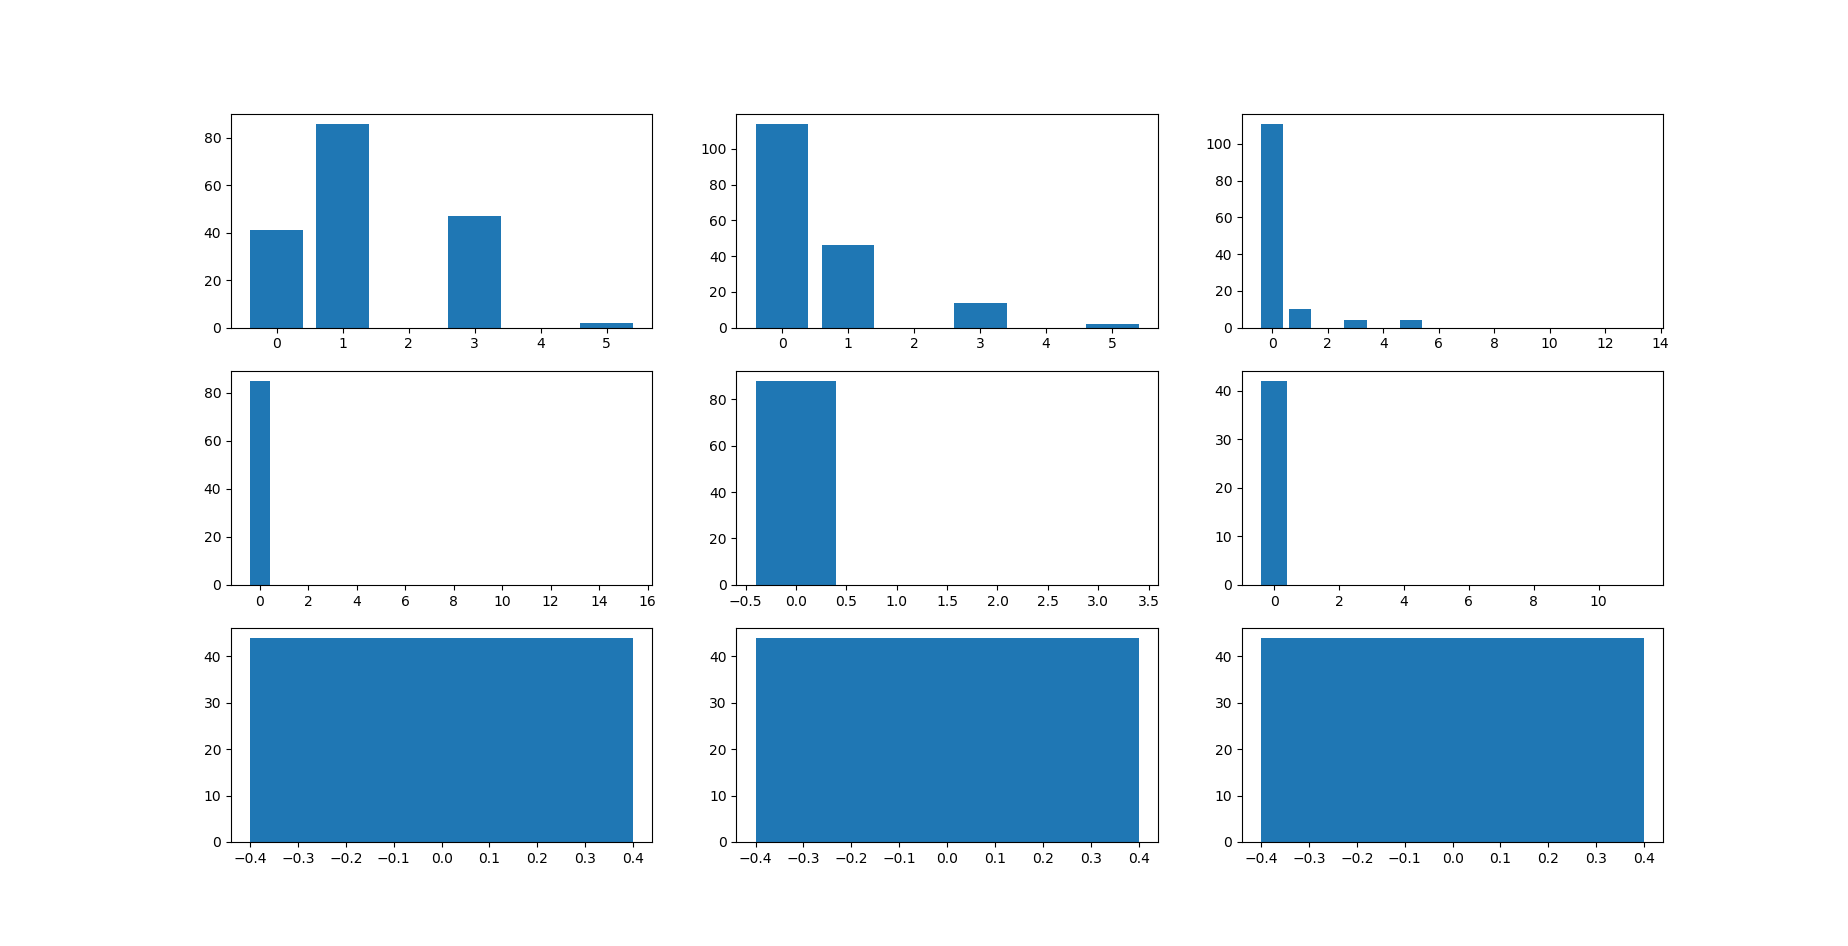
\includegraphics[width=\textwidth]{trefoil_bar.png}
  \caption{Result of the experiment on knots with trefoil input}
  \label{fig:knot_results}
\end{figure}

Figure \ref{fig:knot_results} represents the evolution of the knot determinant through the layers of networks. Each of the subgraph represents a layer from 1 on the top left to 9 on the bottom right. On each of the subgraph the bar represents the absolute number of occurences of a determinant for instance at layer 1 we obtained about 40 knots with determinant 0, 85 with determinant 1, 45 with determinant 3 and 5 with determinant 5.\\

Note that using our alorithm unknots have determinant 0 if they are entangled unknots (more than 1 component) and 1 if they are trivial unknots (1 component and 0 crossing).

\subsection{Considerations}

We can see that as layer index increases, the knots become entangled unknots. An interesting following to this research would be to see if it is possible to create a neural network or set of weights that result in a different knot that an entangled unknot. 

\newpage
\thispagestyle{empty}
\mbox{}
\newpage

\section{Extending the study of expressiveness with topological data analysis} 

In this section, we detail the work on using homology for neural entwork expressiveness inspired by the research detailed in \textbf{Section \ref{sec:tda_bib}} where we try to extend the experiment introduced by Guss in \cite{guss_characterizing_2018} to understand quantitatively the influence of a neural network architecture on it capacity to characterizing homologies in different dimension. 

\subsection{Methodology}

\begin{definition}
  Let $(X, D)$ be a metric space with $D : X^2 \to \R^+$. Let $c \in X$ and $r \in \R$.\\
  \\
  $\B(c,r)$ is the topological ball of radius $r > 0 $ centered on $x$:
  \begin{center}
    $\B(c,r) = \{ x \in X \mid D(x,c) \le r \}$ 
  \end{center}
  $\S(c,r)$ is the topological sphere of radius $r > 0$ centered on $x$:
  \begin{center}
    $\S(c,r) = \{ x \in X \mid D(x,c) = r \}$ 
  \end{center}
  $\mathfrak{S}(c,[r_1,r_2])$ is the thick sphere of border ranging from $r_1$ to $r_2 \ne 0$ ($0 \le r1 \le r_2$) centered on $x$:
  \begin{center}
    $\mathfrak{S}(c,[r_1, r_2]) = \{ x \in X \mid r1 \le D(x,c) \le r_2 \}$ 
  \end{center}
  \label{def:ball_sphere}
\end{definition}

Note that a ball is a particular case of thick sphere where $r_1 = 0$ and spheres are thick spheres with $r_1 = r_2$. Thick sphere is unlike spheres and balls not a rigorous term of topology since it is always equivalent to a sphere or a ball but it is the concept we will use to informatically modelize our balls and spheres.\\

Let $n \in \N^*$, we will consider $X = \R^n$ containing $N_B$ balls $\B_i, 1 \le i \le nB$ and $N_S$ spheres or thick sphere $\S_j, 1 \le j \le N_S$ (cf Definition \ref{def:ball_sphere}) of dimension at most $n$. We informatically modelize this set in the following manner: \\ 

We used datasets of 50000 points split in two non-intersecting classes labelled "0" and "1". The points of class "1" are uniformly spread across various topological spheres and balls. In our case uniformly will mean that the points are uniformly distributed across the volume of the topological feature and that the number of points in each topological feature is proportional to its importance in the sum of volumes of topological features in our set of interest. \\

The points of class "0" are distributed uniformly in the space $X \backslash \{\bigcup\limits_{i=1}^{N_B} \B_i \bigcup \bigcup\limits_{j=1}^{N_S} \S_i \}$.\\

For the result that we will present in \textbf{Section \ref{sec:homology_results}}. We trained network on twelve different sets of dimension 2, 3 and 4 with one to three topological features. On each of these sets we trained 20 sets of fully-connected networks of width 8 and depth 1,2,4,6,8,10,12,14,16 with random initialization for 2000 epochs. To train the networks we used the sparse categorical entropy as loss function, a batch size of 10 and the Adam optimizer with 80\% of the data used as training data and 20\% as validation data. We used Keras \cite{chollet2015keras} with a tensorflow backend in python3. 


\subsection{Algorithms}

In this section we introduce the different algorithm implemented for the research described in this section. All the algorithm have been implemented in python and can be found in the code available on Gitlab \url{https://gitlab.com/Spiilgriim/nnexpy} and the file and line to look for the python file including the implementation can be found in the algorithm title.\\

First we will detail the algorithm to generate our datasets consisting of balls and spheres. Denote $n \ge 2$ the dimension of the space, 

\begin{center}
 $B = \{(\B(c_i, r_i), d_i, o_i)\}_{1 \le i \le N_B}$ 
\end{center}

 the set of balls in $X$ as well as their dimension $d_i$ and orientation $o_i$. Finally

 \begin{center}
  $S = \{(\mathfrak{S}(c_j, [r_{1_j}, r_{2_j}]), d_j, o_i)\}_{1 \le j \le N_S}$ 
 \end{center}

the set of thick sphere and P the number of points in each class. The orientation of balls and spheres is an array of that indicates the index of the elements of the cannonical basis constituing the hyperplane of $\R^n$ in which the feature does not live. For instance in $\R^3$ writting the cannonical basis $\{(1,0,0), (0,1,0), (0,0,1)\}$, $(\B(0,1),2,[1])$ is a 2-dimensional ball centered at the point $(0,0,0)$ of radius $1$ and living in the plane spanned by $\{(0,1,0),(0,0,1)\}$. In the python implementation some of the parameters might be decided randomly or with the help of other parameters.\\

In the algorithm $z$ will refer to a random number between 0 and 1.

\begin{algorithm}[H]
  \begin{algorithmic}[1]
    \STATE points $\gets []$
    \STATE $X \gets S$
    \FOR{$\B_i \in B$}
    \STATE $X \gets X::(\mathfrak{S}(c_i, [0, r_i]), d_i, o_i)$
    \ENDFOR
    \STATE sum $\gets 0$
    \FOR{$i = 1$ to $N_B + N_S$}
    \STATE sum $\gets \text{sum}+ {r_{i_1}}^{d_i} - {r_{i_2}}^{d_i}$
    \ENDFOR
    \FOR{$i = 1$ to $N_B + N_S$}
    \FOR{$j = 1$ to $\lfloor \frac{{r_{i_1}}^{d_i} - {r_{i_2}}^{d_i}}{sum} \rfloor$}
    \STATE temp $\gets 0_{\R^n}$
    \STATE radius $ \gets (r_{i_1} * z_1 + r_{i_2} * (1 - z_1))$
    \FOR{$e = 1$ to $n$}
    \IF{$e \notin o_i$}
    \STATE temp$_i \gets (2*z_2 - 1)$
    \ENDIF
    \ENDFOR
    \STATE points $\gets$ points$::\frac{\text{radius}}{\sqrt{\sum\limits_{i=1}^n \text{temp}_i}} \times \text{temp}$
    \ENDFOR
    \ENDFOR
    
  \end{algorithmic}
  \caption{Generation of topological features \\ ({\fontfamily{cmtt}\selectfont nnexpy/homology\_data\_generation.py l.191})}
  \label{alg:topo_gen}
\end{algorithm}

We have also designed an algorithm to compute betti numbers for spheres and balls that is a more efficient than persistent homology memory-wise due to the limitation to simple topological features. We write $T \in \R^+$ the threshold chosen to compute betti numbers, it corresponds to the radius up to which imaginary balls around each point grow in the persistent homology algorithm. We denote $G$ a graph, $C(G)$ the list of connected components of $G$, $M(X)$ the matrix corresponding to the concatenation of the points of the set $X$ and we extend the definition of $D: X \times A \to \R$ with $A$ a subset of $X$ as $D(x,A) = \underset{y \in A}{\min}$ $D(x,y)$.

\begin{algorithm}[H]
  \begin{algorithmic}[1]
    \STATE betti $\gets \underbrace{[0 ... 0]}_{n \text{ times}}$
    \STATE $G\_\text{node} \gets$ points
    \STATE $G\_\text{edge} \gets []$
    \FOR{$i,j \in \text{points}$}
    \IF{$d(i,j) \le T$}
    \STATE $G\_\text{edge} \gets G\_\text{edge}::(i,j)$
    \ENDIF
    \ENDFOR
    \FOR{$\mathcal{C} \in C(G)$}
    \STATE compute barycenter $B$ of $\mathcal{C}$
    \IF{$D(\mathcal{C},B) \le T$}
    \STATE betti$_0 \gets$ betti$_0 + 1$
    \ELSE
    \STATE betti$_{rank(\mathcal{C}) - 1} \gets$ betti$_{rank(\mathcal{C}) - 1} + 1$
    \ENDIF
    \ENDFOR
  \end{algorithmic}
\caption{Custom persistent homology ({\fontfamily{cmtt}\selectfont nnexpy/homology\_data\_generation.py l.414})}
\end{algorithm}

\subsection{Results}

\label{sec:homology_results}

In Table \ref{tab:betti_res} and Table \ref{tab:bottleneck_res}, one can see the results obtained for the experiments described in this section. 

\begin{table}[H]
  \centering
  \begin{adjustbox}{angle=-90}
  \begin{tabular}{|c|c|c|c|c|c|c|c|c|c|c|c|}
    \hline
    \diagbox{depth}{betti} & [3,0] & [1,1] & [1,0] & [0,0,1] & [0,1,0] & [1,1,0] & [1,0,1] & [0,0,0,1] & [0,0,1,0] & [1,0,1,0] & [1,0,0,1]\\
    \hline
    1 & 13 & 12 & 11 & 15 & 13 & 4 & 2 & 19 & 20 & 13 & 9\\
    \hline
    2 & 18 & 19 & 2 & 19 & 15 & 14 & 12 & 17 & 19 & 18 & 6\\
    \hline
    4 & 18 & 19 & 5 & 17 & 12 & 12 & 14 & 17 & 20 & 19 & 13\\
    \hline
    6 & 19 & 17 & 1 & 19 & 15 & 14 & 13 & 18 & 20 & 20 & 14\\
    \hline
    8 & 17 & 15 & 2 & 18 & 15 & 14 & 19 & 17 & 20 & 20 & 15\\
    \hline
    10 & 15 & 13 & 1 & 19 & 13& 14 & 18 & 18 & 19 & 18 & 10\\
    \hline
    12 & 15 & 10 & 2 & 16 & 9 & 13 & 17 & 16 & 20 & 17 & 13\\
    \hline
    14 & 16 & 9 & 1 & 14 & 7 & 12 & 15 & 16 & 17 & 14 & 10\\
    \hline
    16 & 10 & 6 & 1 & 7 & 6 & 12 & 10 & 13 & 12 & 13 & 8\\
    \hline
  \end{tabular}
\end{adjustbox}
    \caption{The number of occurences of the same betti numbers between the original data persistence diagram and the networks data persistence diagram}
    \label{tab:betti_res}
\end{table}


\begin{table}[H]
  \centering
  \begin{adjustbox}{angle=-90}
  \begin{tabular}{|c|c|c|c|c|c|c|c|c|c|c|c|}
    \hline
    \diagbox{depth}{betti} & [3,0] & [1,1] & [1,0] & [0,0,1] & [0,1,0] & [1,1,0] & [1,0,1] & [0,0,0,1] & [0,0,1,0] & [1,0,1,0] & [1,0,0,1]\\
    \hline
    1 & 0.077 & 0.088 & 0.033 & 0.035 & 0.038 & 0.137 & 0.137 & 0.025 & 0.031 & 0.198 & 0.181 \\
    \hline
    2 & 0.033 & 0.058 & 0.016 & 0.021 & 0.035 & 0.046 & 0.079 & 0.025 & 0.027 & 0.110 & 0.125 \\
    \hline
    4 & 0.023 & 0.019 & 0.011 & 0.019 & 0.043 & 0.050 & 0.034 & 0.025 & 0.029 & 0.051 & 0.054 \\
    \hline
    6 & 0.013 & 0.012 & 0.006 & 0.020 & 0.040 & 0.035 & 0.024 & 0.024 & 0.024 & 0.035 & 0.059 \\
    \hline
    8 & 0.025 & 0.011 & 0.010 & 0.017 & 0.042 & 0.041 & 0.019 & 0.028 & 0.028 & 0.050 & 0.041 \\
    \hline
    10 & 0.028 & 0.016 & 0.006 & 0.019 & 0.039 & 0.036 & 0.024 & 0.028 & 0.026 & 0.056 & 0.047 \\
    \hline
    12 & 0.031 & 0.009 & 0.007 & 0.018 & 0.043 & 0.041 & 0.023 & 0.026 & 0.032 & 0.051 & 0.071 \\
    \hline
    14 & 0.023 & 0.010 & 0.007 & 0.019 & 0.041 & 0.042 & 0.021 & 0.023 & 0.027 & 0.040 & 0.067 \\
    \hline
    16 & 0.025 & 0.020 & 0.012 & 0.020 & 0.044 & 0.041 & 0.024 & 0.023 & 0.034 & 0.055 & 0.046 \\
    \hline
  \end{tabular}
\end{adjustbox}
    \caption{The average bottleneck distance between the original data persistence diagram and the networks data persistence diagram}
    \label{tab:bottleneck_res}
\end{table}

\subsection{Considerations}

In table \ref{tab:betti_res} we can see a tendency for the number of proper characterizations to first go up since the network gets deeper and more expressive as expected and then down. The drop in the number of proper characterizations is due to the difficulty to train big networks since they would require more epochs than used but we could not for time reasons allocate more time to the network training considering how long the process is. Another problem we faced in the case where the topological feature only live in a strict subspace of $X$ is that we might see the appearance of training artifacts in the region where there should be no points. This causes the computation of betti numbers to return a result different from the original one because it changes the dimension in which the feature lives in.\\

Finally another problem with this experiment is the time required to train enough networks and train them properly. To reproduce Guss' experiment described in \textbf{Section \ref{sec:tda_bib}} with only 2000 epoch of training on an NVIDIA RTX 2080 and 16 GB of RAM we would need approximately 50 days of uninterrupted computation. The results obtained with the various training are yet insufficent to draw any significant conclusion but with the availability of the code and its documentation should allow anyone with enough computation power to run statistically significant experiments and draw the numeric conclusion.\\

\newpage
\thispagestyle{empty}
\mbox{}
\newpage

\bibliography{bibliography}

\bibliographystyle{ieeetr}

\newpage
\thispagestyle{empty}
\mbox{}
\newpage

{\LARGE \textbf{Acknowledgements}}

\vspace{20mm}

\textit{Thanks to my family and friends for their constant support through my research}\\

\textit{Merci à ma famille et mes amis pour leur soutient sans faille pendant mes recherches}\\

\begin{CJK}{UTF8}{min} 私の研究を通して絶え間ないサポートをしてくれた家族や友人に感謝します  \end{CJK} (Maybe better translation required)\\

\newpage
\thispagestyle{empty}
\mbox{}
\newpage

\section{Appendix}

\subsection{Figures credit}
\begin{figure}[H]
  \centering
  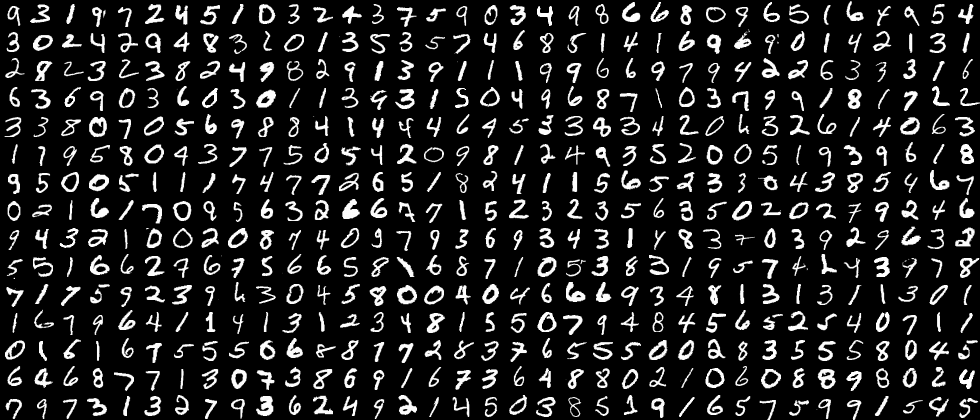
\includegraphics[width=.3\textwidth]{mnist.png}
  \caption[]{By Josef Steppan - Own work, CC BY-SA 4.0, https://commons.wikimedia.org/w/index.php?curid=64810040}
\end{figure}

\begin{figure}[H]
  \centering
            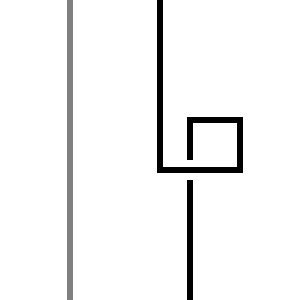
\includegraphics[height=100pt]{r1.png}
            \caption[]{Parcly Taxel- Own work, FAL, https://commons.wikimedia.org/w/index.php?curid=68523335}
\end{figure}
\begin{figure}[H]
             \centering
            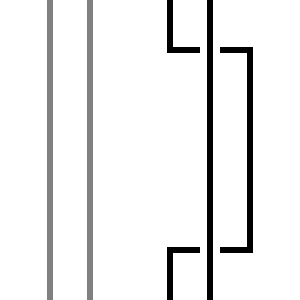
\includegraphics[height=100pt]{r2.png}
            \caption[]{By Parcly Taxel- Own work, FAL, https://commons.wikimedia.org/w/index.php?curid=68523334}
\end{figure}
\begin{figure}[H]
             \centering
            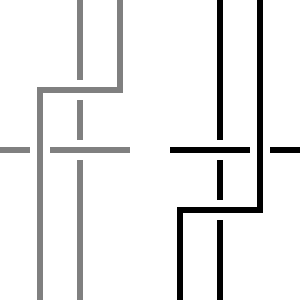
\includegraphics[height=100pt]{r3.png}
            \caption[]{By Parcly Taxel- Own work, FAL, https://commons.wikimedia.org/w/index.php?curid=68523336}
\end{figure}

\begin{figure}[H]
  \centering
  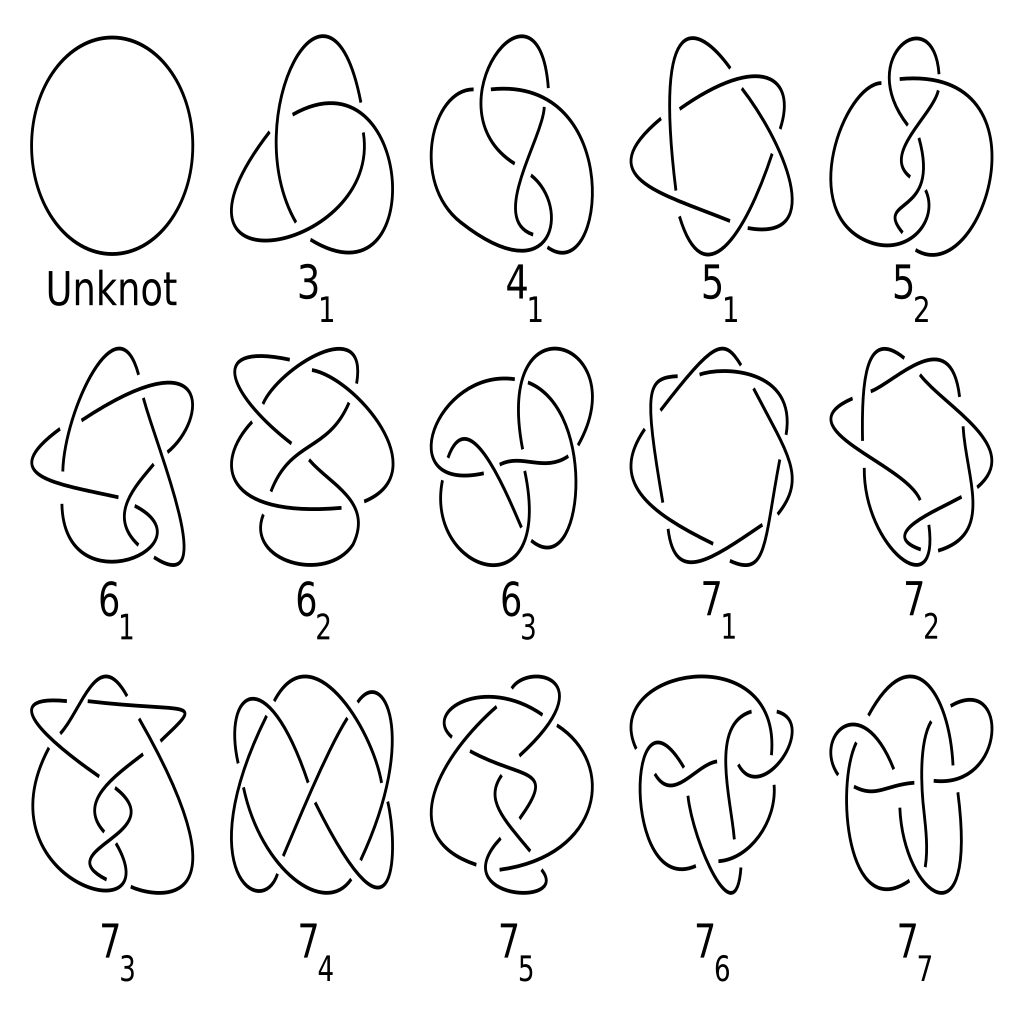
\includegraphics[width=.6\textwidth]{knot_table.png}
  \caption[]{By Jkasd - Own work, Public Domain, https://commons.wikimedia.org/w/index.php?curid=3937733}
\end{figure}

\begin{figure}[H]
  \begin{minipage}[c]{.2\textwidth}
  \centering
  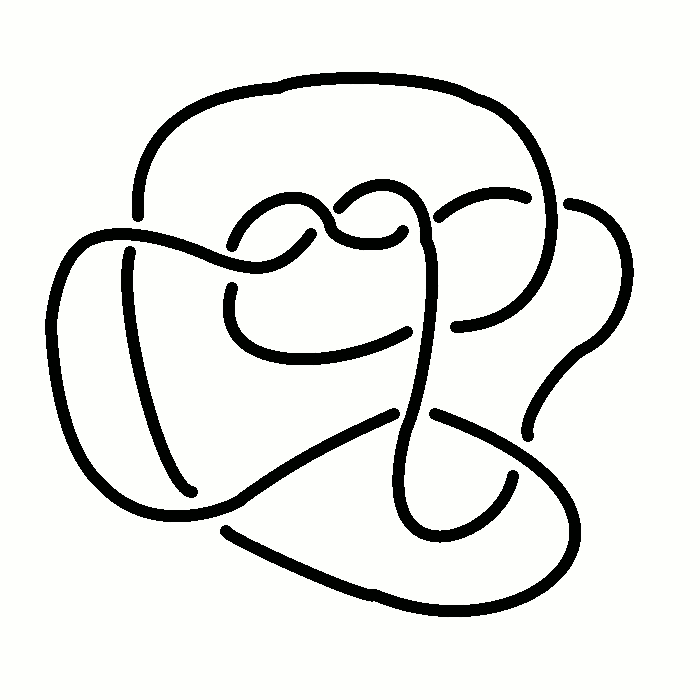
\includegraphics[width=.95\textwidth]{knot_unfolding-0.png}
    
  \end{minipage}
  \hfill
  \begin{minipage}[c]{.2\textwidth}
  \centering
  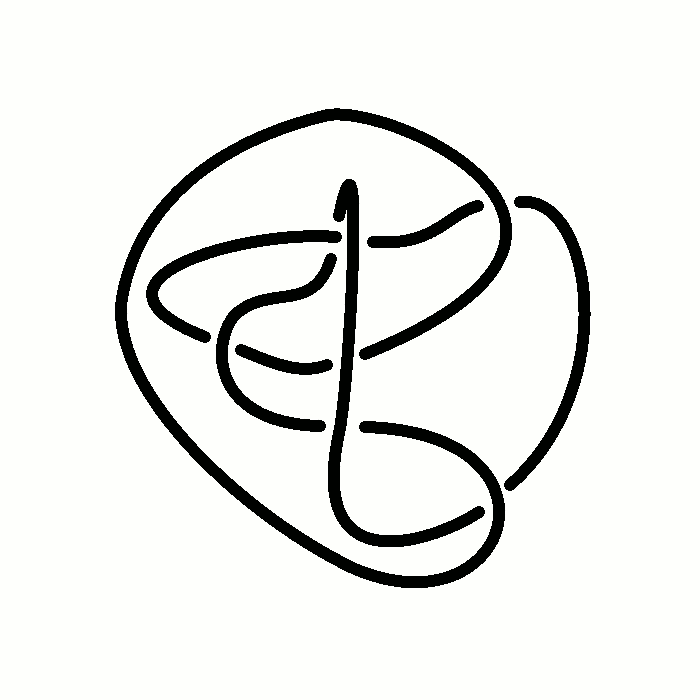
\includegraphics[width=.95\textwidth]{knot_unfolding-10.png}
    
  \end{minipage}
  \hfill
  \begin{minipage}[c]{.2\textwidth}
  \centering
  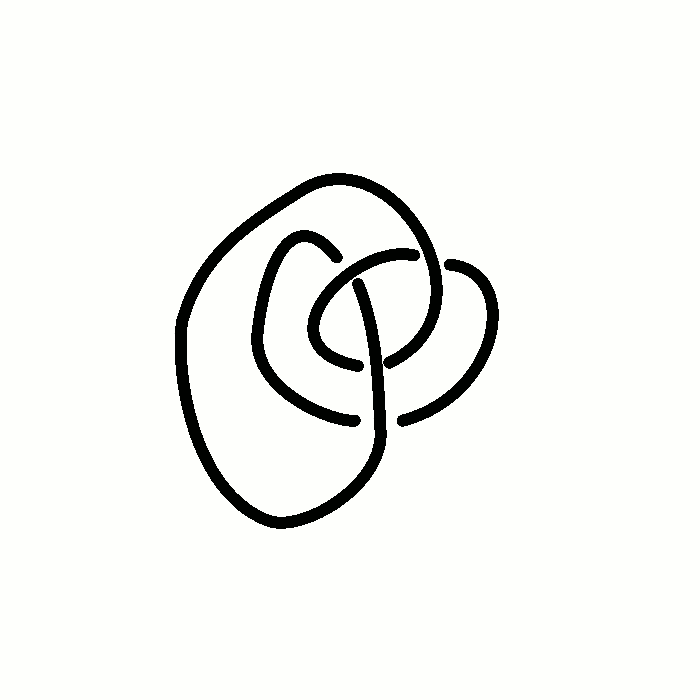
\includegraphics[width=.95\textwidth]{knot_unfolding-20.png}
    
  \end{minipage}\\
  \begin{minipage}[c]{.2\textwidth}
  \centering
  \includegraphics[width=.95\textwidth]{knot_unfolding-30.png}
    
  \end{minipage}
  \hfill
  \begin{minipage}[c]{.2\textwidth}
  \centering
  \includegraphics[width=.95\textwidth]{knot_unfolding-40.png}
    
  \end{minipage}
  \hfill
  \begin{minipage}[c]{.2\textwidth}
  \centering
  \includegraphics[width=.95\textwidth]{knot_unfolding-50.png}
    
  \end{minipage}
  \caption[]{By Kuchtact - Own work, CC BY-SA 4.0, https://commons.wikimedia.org/w/index.php?curid=77971069}
\end{figure}

\begin{figure}[H]
  \centering
  \includegraphics[width=.3\textwidth]{trefoil_nat.png}
  \caption[]{By Marnanel - Image:TrefoilKnot-01.png, Public Domain, https://commons.wikimedia.org/w/ index.php?curid=3246080}
\end{figure}

\begin{figure}[H]
  \centering
  \includegraphics[width=.3\textwidth]{fig_eight_nat.png}
  \caption[]{ By Talifero - File:Knots eight shamrock.svg, Public Domain, https://commons.m.wikimedia.org/wiki/File:Knots eight shamrock.svg}
\end{figure}
\end{document}

